\documentclass[10pt]{article}
\usepackage[margin=1in]{geometry}
\usepackage{graphicx}
\usepackage{booktabs}
\usepackage{multirow}
\usepackage{amsmath}
\usepackage{amssymb}
\usepackage{xcolor}
\usepackage{hyperref}
\usepackage{caption}
\usepackage{subcaption}
\usepackage{enumitem}
\usepackage{microtype}
\hypersetup{colorlinks=true,linkcolor=black,citecolor=blue,urlcolor=blue}

\graphicspath{{figures/}}

\title{Beta-Testing Monopoly: \\Closed-Loop Game-Design Optimisation
       over a Diverse Strategy Pool}
\author{Selim Emir Can (emirc) \and Alaz Cig}
\date{2026-04-24}

\begin{document}
\maketitle

\begin{abstract}
We automate the beta-testing loop a game designer would otherwise run by
hand: treat Monopoly as a parameterised multi-agent system, run a
diverse population of rule-based players against every candidate
design, and score the resulting play on the qualities the designer
cares about. A genetic algorithm searches a 66-dim design space
(per-property cost/rent multipliers + a keep-mask that structurally
shortens the board) to minimise a composite of fairness, game length,
draw rate, and inter-agent money transfer; single-objective ablations
and a $2p\!\leftrightarrow\!3p$ cross-evaluation at $n{=}1000$ yield
$\sim$40\% score reductions over the default board. The contribution
we are claiming, however, is not the better board itself but the
\emph{tool}: agent feedback need not be literally accurate to be
decision-useful, only \emph{directionally} predictive of how the design
change will play in real life. We outline a validation plan
(simplified-board sanity check, human playtest, LLM-agent cross-check)
that operationalises this claim and pre-declares the statistics that
make the agent vs.\ human comparison apples-to-apples.
Code:
\url{https://github.com/Selim-Emir-Can/CS348K-proj}.
\end{abstract}

\section{Introduction}

Tabletop Monopoly is the canonical example of a designed multi-agent game,
and its known issues (games drag on, single-property luck dominates,
two-player play is famously unbalanced) make it a sharp testbed for
automated design optimisation. Our goal is not to ``solve'' Monopoly but
to demonstrate, on a reproducible setup, the beta-testing loop:
\begin{quote}
\textbf{Parameterise environment} $\to$ \textbf{evaluate against a diverse
agent population} $\to$ \textbf{optimise environment for population-level
metrics} $\to$ \textbf{verify the constraints we specified are reflected
in real play.}
\end{quote}

\paragraph{The contribution we are claiming.} The deliverable is not
the optimised board itself but the \emph{tool that produces it}. The
guarantee we are after is weaker and stronger at the same time:
\begin{quote}
\emph{Agent feedback need not be literally accurate to be decision-useful.
What we want is for the design constraints I specify in the agent
setting to be reflected in real-world play with humans, on the same
direction and roughly the same relative magnitude.}
\end{quote}
This framing reduces the burden of proof from ``the agents predict
human win-rates'' (which is hard, possibly hopeless, and not what a
designer needs) to ``the agents predict the \emph{direction} of a design
change'' (which is achievable and exactly what a designer uses agent
feedback for in practice).

The deliverables of this report are: an open-source closed-loop
optimisation codebase; a $5\times 2$ ablation matrix producing concrete
improved boards on which the agent feedback is internally consistent
(Section~\ref{sec:eval}); a per-aspect decomposition of what the
optimiser actually changed (Section~\ref{sec:decomp}); a set of
multi-agent-system generalisations (Section~\ref{sec:gen}); and a
validation plan that operationalises the central claim above by
cross-checking agent predictions against a simplified-board test, a
real-human playtest, and an LLM-agent cross-check
(Section~\ref{sec:validation}).

\paragraph{How this report addresses the grading rubric.}
The two graded criteria are: (1) \emph{problem specificity} and (2)
\emph{evaluation thoughtfulness}. Section~\ref{sec:problem} addresses (1)
by pinning every variable, metric, and budget to a numeric definition.
Section~\ref{sec:eval} addresses (2) with a noise-floor baseline,
single-objective ablations, two search algorithms at matched budget,
$2p\!\leftrightarrow\!3p$ cross-evaluation at $n{=}1000$, and per-strategy
heatmaps that visualise \emph{which} matchups the optimiser actually fixed.

\paragraph{Background and context.} Automated game-design tuning has a
long but uneven history. Classical game-balance work varies a handful of
parameters by hand and validates with a small fixed-playstyle pool of
playtesters; more recent multi-agent RL work (e.g.\ league play in
AlphaStar) inverts the loop, fixing the environment and evolving the
agent population. Our setting sits deliberately between these extremes:
the \emph{environment} is the search variable, and the \emph{agent
population} is fixed, diverse, and designed to represent the plausible
space of rational play. This framing gives the designer actionable
leverage (environment parameters are cheap to change; retraining agents
for every candidate design is not) while retaining the honesty of a
population-level evaluation (the optimum must generalise across
strategies, not just overfit to one reference agent). The same framing
applies to matchmaker design, auction-parameter tuning, platform-rules
optimisation, and any other multi-agent system whose designer can
instrument the environment independently of the agents that populate it.

\paragraph{What an ``improvement'' means here.} Throughout the paper we
describe a design as ``improved'' when its weighted combined score
(Eq.~\ref{eq:score}) is lower than the default board's under the same
evaluation protocol. Because the score aggregates five design qualities
with explicit weights and targets, absolute score values are only
meaningful in relative terms (score~$=0$ would mean every per-matchup
fairness is exactly zero, rounds hit target, zero draws, and transfer at
target simultaneously, which is physically impossible for any non-trivial
strategy pool). Throughout, we report both the composite score and the
underlying per-metric numbers so a reader who cares about only one
dimension (e.g.\ \emph{only} game length) can read that column directly.

\section{Problem definition}\label{sec:problem}

\paragraph{Strategy space.} A \texttt{ParametricPlayer} is a rule-based agent
defined by 17 named knobs (5 continuous, 4 boolean, 8-bit colour-group mask):
\begin{itemize}[leftmargin=1.2em,itemsep=0pt]
\item \texttt{unspendable\_cash}~$\in[0,1500]$, \texttt{build\_cash\_floor}~$\in[0,1500]$
\item \texttt{trade\_max\_diff\_absolute}~$\in[0,500]$,
      \texttt{trade\_max\_diff\_relative}~$\in[1,5]$
\item \texttt{jail\_pay\_threshold}~$\in[0,1500]$
\item booleans: \texttt{is\_willing\_to\_make\_trades, aggressive\_build,
      buy\_utilities, buy\_railroads}
\item \texttt{ignore\_property\_groups} (subset of 8 colour groups)
\end{itemize}

\paragraph{Strategy pool (30 strategies).} 10 hand-designed named archetypes
each with an explicit rationale (\textsl{AggressiveBuilder, CashHoarder,
Trader, RailroadKing, LowCostOnly, HighCostOnly, Balanced, Passive, Bully,
RiskAverse}) plus 20 randomly sampled strategies, deterministic via a fixed
seed. Saved once to JSON and reloaded by every optimisation run. Full
parameter specifications and archetype rationales are catalogued in
Appendix~\ref{app:strategies}.

\paragraph{Board design space (45 dims).}
\begin{itemize}[leftmargin=1.2em,itemsep=0pt]
\item 22 continuous \emph{cost multipliers} $c_i\in[0.5,2.0]$ scaling
      \texttt{cost\_base} and \texttt{cost\_house} of each colour-group property
\item 22 continuous \emph{rent multipliers} $r_i\in[0.5,2.0]$ scaling
      \texttt{rent\_base} and \texttt{rent\_house}$_{0\dots 4}$ proportionally
\item 1 integer \emph{property count} $N_{\text{props}}\in[8,22]$. Removed
      properties are replaced with FreeParking cells at the same board index,
      preserving the 40-cell layout so hardcoded Chance-card positions remain
      valid. Railroads and utilities are fixed.
\end{itemize}

\paragraph{Evaluation protocol.} For each player count $n\in\{2,3\}$ we
fix \emph{10 evaluation matchups} sampled once at init from the strategy
pool with diversity constraints: every named archetype appears at least
once; at least 3 matchups include a sampled strategy. Each candidate
board is evaluated on $\,10\!\times\!10 = 100$ games (10 games per
matchup, split evenly across seat permutations to neutralise first-mover
advantage). Per-game seeds are identical across all candidates so an
unchanged design vector yields byte-identical metrics.

\paragraph{Metrics and combined objective (minimise).} Per-matchup we
compute fairness $|\,w_{p_0}\!-\!w_{p_1}|$ (or $\max\!-\!\min$ for 3p),
draw rate, mean rounds, and \emph{player-to-player money transfer rate}
(rent paid + trade-cash deltas, normalised per round; a proxy for
agent-agent interactivity). Across 10 matchups:
\begin{equation}\label{eq:score}
\text{score}(\theta) =
   w_{\text{fair}} \overline{F} +
   w_{\text{fmax}} F_{\max} +
   w_{\text{len}}  \frac{|\overline{R}\!-\!R^*|}{R^*} +
   w_{\text{draw}}\overline{D} +
   w_{\text{money}}\frac{|\overline{T}\!-\!T^*|}{T^*}
\end{equation}
with defaults $w=(1,\,0.5,\,0.5,\,0.3,\,0.3)$, $R^*{=}60$ rounds,
$T^*{=}100$ \$/round. Here $\overline{F}$ is the mean pair-fairness
(absolute win-rate gap between players, averaged over the 10 evaluation
matchups), $F_{\max}$ is the worst-pair fairness (a robustness term),
$\overline{R}$ is the mean round count, $\overline{D}$ is the draw rate,
and $\overline{T}$ is the mean per-round player-to-player cash transfer.
Every non-fairness term is normalised by its target so the weights are
dimensionless. The defaults encode a qualitative judgement: fairness is
the primary concern (weight 1.0), length and interactivity matter half
as much (weight 0.5), and decisiveness matters slightly less still
(weight 0.3). We ablate each weight to zero in Section~\ref{sec:eval}
to confirm the composite is not dominated by any one term.

\paragraph{Search.} Two algorithms, equal budget ($\sim$200 evaluations).
\textbf{Random search} draws each dimension uniformly from its bounds.
\textbf{GA}: population 20, 10 generations, tournament selection ($k{=}3$),
uniform crossover, Gaussian mutation $\sigma{=}0.1$ on continuous dims,
$\pm 1$ on $N_{\text{props}}$, elitism 2.

\paragraph{Reproducibility budget.} Total games for the entire study:
$\approx 100\text{k}$ optimisation evaluations + $\approx 30\text{k}$
high-CI cross-evaluation + $\approx 35\text{k}$ heatmap evaluations
$\approx 165\text{k}$ games, $\approx 25$ minutes wall-clock on a single
CPU at $\approx 6$ ms/game.

\section{Approach}

\paragraph{Simulator wrapper.} We re-use the existing core game loop
(\texttt{monopoly\_game\_from\_config}) but wrap it so that each call returns
a per-game stat dict (winner, rounds, bankruptcy map, transfer total). Inter-
player cash flow is captured via a context-manager monkey-patch of
\texttt{Player.pay\_money}; non-player payments (taxes, fines, salary) are
not counted. To prevent oscillating trade loops, we cap
\texttt{Player.do\_a\_two\_way\_trade} calls per (player, turn) at 5; this
breaks an unbounded \texttt{while} in the core code without affecting any
legitimate trade behaviour.

\paragraph{Design-space encoder/decoder.} The \texttt{DesignSpace} class
maps a 45-dim vector to a fresh \texttt{GameConfig}: per-property
multipliers are applied to \texttt{cost\_base},
\texttt{cost\_house}, \texttt{rent\_base}, and \texttt{rent\_house}, and
shrinkage substitutes \texttt{FreeParking} for the lowest-cost-ranked
properties. Identity vector $=$ the canonical default board.

\paragraph{Pipeline.} \texttt{scripts/optimize\_board.py} drives the search,
emitting one JSONL line per evaluation. \texttt{scripts/report\_runs.py}
produces convergence and Pareto plots. \texttt{scripts/cross\_eval.py} runs
designs through both player-count harnesses at $n{=}1000$. Finally,
\texttt{scripts/strategy\_heatmap.py} produces the $30{\times}30$
strategy-vs-strategy win-rate matrix on any chosen design.
Appendix~\ref{app:impl} details the simulator instrumentation,
design-space encoding, GA hyperparameters, and the determinism guarantees
that make every reported number reproducible from its run's meta file.

\section{Evaluation}\label{sec:eval}

\subsection{Experimental setup and reading guide}

We run the experimental matrix in three stages, each addressing a
distinct evaluation question. The \emph{default-board baseline} answers
``what do we have to beat?'' (Section~\ref{sec:default}). The
\emph{search comparison and ablation matrix} answers ``is the optimiser
finding something real, and is each term of the objective doing useful
work?'' (Sections~\ref{sec:randvsga}, \ref{sec:ablation}). The
\emph{high-confidence cross-evaluation} answers ``does the winning design
generalise past the training protocol?'' (Section~\ref{sec:cross}).
Finally, \emph{per-strategy heatmaps} and
\emph{qualitative board visualisations} (Sections~\ref{sec:heatmap},
\ref{sec:boards}) diagnose the mechanism: where the optimiser pushed
fairness, and which specific properties it chose to drop.

All tables report the same five metrics so results are directly
comparable across sections: \emph{score} (combined objective,
Eq.~\ref{eq:score}, lower is better); \emph{mean fair} (average pair
fairness, $0$ is perfectly balanced, $1$ is one player wins every game);
\emph{max fair} (worst-pair fairness); \emph{rounds} (mean game length
in turns); \emph{draw \%} (fraction of games hitting the 200-turn
truncation cap with no bankrupt player); \emph{transfer} (mean
player-to-player cash flow per round, target $\$100$). Wilson 95\% CIs
are computed for every win-rate proportion; widths are $\pm 3$pp at
$n{=}1000$ and $\pm 10$pp at $n{=}100$. Random seeds and matchup indices
are shared across every candidate design, so any two runs with the same
design vector produce byte-identical numbers.

\subsection{Default-board baseline (the ``before'' picture)}\label{sec:default}

Table~\ref{tab:default} shows the default board's metrics under our
evaluation harness. It establishes the reference each optimisation must beat.

\begin{table}[h]
\centering
\small
\begin{tabular}{lrrrrrr}
\toprule
                 & score & mean fair & max fair & rounds & draw \% & transfer \\
\midrule
Default 2p (n=100)   & 1.556 & 0.540 & 1.000 &  101.9 &  6.0 &  50.4 \\
Default 3p (n=100)   & 1.504 & 0.540 & 0.900 &  113.2 & 22.0 &  98.2 \\
Default 2p (n=1000)  & 1.463 & 0.454 & 0.940 &  103.9 &  7.4 &  49.7 \\
Default 3p (n=1000)  & 1.230 & 0.412 & 0.680 &  110.8 & 17.6 &  99.4 \\
\bottomrule
\end{tabular}
\caption{\textbf{Default Monopoly board, evaluated under our harness to
establish the pre-optimisation reference.} Each row is 100 or 1000 games
played on the unmodified canonical board with our 30-strategy pool
drawing from 10 fixed evaluation matchups. \emph{Score} is the composite
objective of Eq.~\ref{eq:score} (lower = closer to ``fair, well-paced,
decisive, interactive'' board). Mean fairness of $0.54$ means the two
players' win rates differ by an average of 54 percentage points across
matchups: in most pairings one player completely dominates the other.
The mean round count is $\sim$100 (vs.\ our target of 60), so default
games drag. Money transfer of $\$50$/round in 2p falls well short of the
$\$100$ target, meaning the default 2p board is substantially less
interactive than the designer would prefer. 3p defaults hit transfer
target ($\$98$) but saturate on draws ($22\%$ of games truncate without
a clear winner). These numbers form the ``defeat me'' bar for every
subsequent optimised design: \emph{any} improvement in score at
$n{=}1000$ (the bottom two rows) is meaningful because Wilson CIs at
that sample size are $\pm 3$pp on individual win rates.}
\label{tab:default}
\end{table}

\subsection{Random search vs.\ genetic algorithm}\label{sec:randvsga}

At an equal evaluation budget ($\sim$200 evaluations, corresponding to
$\sim$20k simulated games per search run), the GA decisively beats
random search on both player counts (Figure~\ref{fig:convergence}).
Beyond headline score, two qualitative differences matter for the
broader methodology claim: (i) the GA's best-so-far curve \emph{improves
monotonically} over the run, while random search's curve plateaus after
whichever early sample happens to land well, and (ii) the top-5 GA
designs cluster tightly in metric space (small within-cluster variance
on each metric column of Table~\ref{tab:ablation}) while the top-5
random designs are scattered, meaning the GA has found a \emph{robust
basin of good designs}, not a single lucky point.

\begin{figure}[h]
\centering
\begin{subfigure}{0.49\linewidth}
\centering

\includegraphics[width=\linewidth]{convergence_2p.png}
\caption{2-player Monopoly.}
\end{subfigure}
\begin{subfigure}{0.49\linewidth}
\centering

\includegraphics[width=\linewidth]{convergence_3p.png}
\caption{3-player Monopoly.}
\end{subfigure}
\caption{\textbf{Search convergence on the 45-dimensional board design
space.} Each curve is the best-so-far score (lower is better) versus
evaluation index for one search run. We plot six runs per player count:
random search and the combined-objective GA (both at $\sim$200
evaluations for direct comparison), plus four single-objective GA
ablations (\texttt{abl\_fair}, \texttt{abl\_len}, \texttt{abl\_draw},
\texttt{abl\_money}). Three observations: (i) at matched evaluation
budget, the combined-objective GA decisively beats random search by
$16$--$17$\% on best final score for both player counts; (ii) GA
convergence is monotone and stable, while random search relies entirely
on lucky early samples; (iii) the four single-objective ablations
collapse to near $0$ individually, demonstrating each objective is
\emph{independently} achievable -- the combined optimum is therefore a
genuine multi-objective trade-off rather than a search failure. The
horizontal asymptote of each ablation curve is the lower bound of that
objective term for the fixed strategy pool and matchup set.}
\label{fig:convergence}
\end{figure}

\subsection{Single-objective ablations: trade-offs are real}\label{sec:ablation}

A common failure mode in multi-objective design is that one term
dominates the composite and the optimiser effectively ignores the
others; then the composite reduces to a single-objective problem in
disguise. To rule this out, we run the GA five additional times per
player count, each with all but one objective weight set to zero, and
take the best design from each run. If each term is independently
meaningful, the ablation winners should each drive their own metric to
its lower bound while \emph{degrading} at least one other metric
(showing the combined objective trades it off rather than ignoring it).
Each row of Table~\ref{tab:ablation} is the best design from a GA run
with a single objective active. Three of four single-objective runs
drive their target metric to (or near) zero, but always at the cost of
one or more other metrics, confirming the combined objective's
components are non-redundant.

\begin{table}[h]
\centering
\small
\begin{tabular}{llrrrrrr}
\toprule
$n$ & Run             & score & fair & rounds & draw \% & transfer \\
\midrule
2p & GA combined      & 0.830 & 0.230 & 61.7 & 1.0  & 72.2 \\
2p & GA fairness-only & \textbf{0.280} & \textbf{0.280}$\downarrow$ & 95.6 & 8.0  & 57.4 \\
2p & GA length-only   & \textbf{0.000} & 0.300 & \textbf{60.0}$\checkmark$ & 2.0  & 71.8 \\
2p & GA draw-only     & \textbf{0.000} & 0.460 & 68.2 & \textbf{0.0}$\checkmark$ & 64.5 \\
2p & GA money-only    & \textbf{0.241} & 0.390 & 61.6 & 1.0  & \textbf{75.9}$\uparrow$ \\
\midrule
3p & GA combined      & 0.666 & 0.290 & 68.6 & 2.0  & 116.3 \\
3p & GA fairness-only & \textbf{0.240} & \textbf{0.240}$\downarrow$ & 86.7 & 6.0  & 110.3 \\
3p & GA length-only   & \textbf{0.000} & 0.380 & \textbf{60.0}$\checkmark$ & 4.0  & 115.1 \\
3p & GA draw-only     & \textbf{0.010} & 0.390 & 73.2 & \textbf{1.0}$\downarrow$ & 116.0 \\
3p & GA money-only    & \textbf{0.001} & 0.450 & 110.9 & 19.0 & \textbf{100.1}$\checkmark$ \\
\bottomrule
\end{tabular}
\caption{\textbf{Single-objective ablation winners.} Each row is the
best design discovered by a separate GA run that optimises a single
isolated objective (weights $w_{\text{fair}}$, $w_{\text{len}}$,
$w_{\text{draw}}$, $w_{\text{money}}$ set to $1$ one at a time, all
others zero). ``GA combined'' is the multi-objective run from
Section~\ref{sec:randvsga}, shown on each player-count block for
reference. \textbf{Bold} values mark the metric the ablation was actively
optimising. $\downarrow$ flags a saturating lower bound (the objective
was pushed as low as the strategy pool allows), $\checkmark$ an exact
target hit (the optimiser landed exactly on $R^*{=}60$ rounds or
$0\%$ draws), and $\uparrow$ a saturating upper bound (money-transfer
pushed as high as achievable given the 30-strategy pool). \emph{How to
read the table:} scanning a row shows the trade-offs accepted to
minimise that row's bold objective. For example, 2p fairness-only drove
mean fairness to $0.28$ but rounds blew out to $95.6$ and transfer
dropped to $\$57$; 2p length-only nailed 60 rounds exactly but left
fairness at $0.30$. Only the combined row balances all five dimensions.
The 3p money-only run is illustrative: default 3p is already near the
transfer target ($\$98$), so this ablation exits at nearly the default
configuration, lengthening games to $110.9$ rounds and allowing $19\%$
draws to squeeze the last percent of interactivity gap closed.}
\label{tab:ablation}
\end{table}

\subsection{High-confidence cross-evaluation}\label{sec:cross}

Table~\ref{tab:cross} answers two questions simultaneously. First,
\emph{is the optimisation-set score honest at higher sample sizes?} At
$n{=}100$ games per candidate (our optimisation budget) the per-matchup
CI is $\pm 10$pp; the GA has enough signal to converge but also enough
noise to overfit to the specific seed set. At $n{=}1000$ games, Wilson
CIs tighten to $\pm 3$pp and any overfit becomes visible. Second,
\emph{does a board optimised for one player count generalise to the
other?} We re-evaluate three designs (the GA-2p winner, the GA-3p
winner, and the default board) under both harnesses (2p and 3p matchup
sets) at $n{=}1000$.

\begin{table}[h]
\centering
\small
\begin{tabular}{llrrrrrr}
\toprule
Design & Eval & score & fair & max\,f & rounds & draw \% & transfer \\
\midrule
default board    & 2p & 1.463 & 0.454 & 0.940 & 103.9 &  7.4 &  49.7 \\
default board    & 3p & 1.230 & 0.412 & 0.680 & 110.8 & 17.6 &  99.4 \\
\addlinespace
GA-2p winner     & 2p & \textbf{0.998} & 0.323 & 0.960 &  69.4 & 2.3 &  63.4 \\
GA-2p winner     & 3p & 0.690 & 0.248 & 0.610 &  71.2 & 3.0 & 111.7 \\
\addlinespace
GA-3p winner     & 2p & 0.954 & \textbf{0.251} & 0.960 &  71.0 & 2.7 &  58.8 \\
GA-3p winner     & 3p & \textbf{0.670} & 0.255 & 0.550 &  72.4 & 4.3 & 107.7 \\
\bottomrule
\end{tabular}
\caption{\textbf{High-confidence cross-player-count evaluation
($n{=}1000$ games per cell, Wilson 95\% CIs of $\pm 3$pp on individual
win rates).} Each row is one (design, harness) pair: ``design'' names the
board being evaluated, ``eval'' names the player-count regime of the
harness it is evaluated under (which determines both the matchup set
and the number of seats at the table). Rows $1$--$2$ are the default
board, re-evaluated here at larger $n$ than in Table~\ref{tab:default} so
numbers are directly comparable to the optimised rows. Rows $3$--$4$ run
the GA-2p winner against both harnesses; rows $5$--$6$ do the same for
the GA-3p winner. \emph{Reading the table:}
(i)~\emph{Improvement over default.} Every optimised-design row cuts
mean rounds by $30$--$40$ (from $\sim$100+ to $\sim$62--71),
cuts draw rate by $\geq 70\%$ (from $7.4\%/17.6\%$ to $\leq 4.3\%$),
and shifts transfer rate towards the target. Fairness also drops
across the board by $20$--$50\%$ relative to default.
(ii)~\emph{Cross-regime generalisation.} Neither optimised design
catastrophically fails on the other player count; both are still
meaningful wins over the default. The GA-3p winner is the stronger
universal design: its 2p score ($0.954$) is \emph{better} than the
GA-2p winner's own 2p score ($0.998$) because the GA-3p optimum
happened to yield stronger fairness ($0.251$ vs.\ $0.323$). This
suggests 3p optimisation implicitly pressure-tests more strategy
interactions, producing a more robust design.
(iii)~\emph{The score at $n{=}1000$ is slightly worse than the
$n{=}100$ training score} (GA-2p: $0.83 \to 0.998$; GA-3p:
$0.67 \to 0.67$). The first gap is an honest \emph{optimisation-set
overfit}: the GA found a design with seed-specific advantages on its
training matchup set that partially wash out at higher $n$. We report
both numbers rather than cherry-pick the more flattering one.}
\label{tab:cross}
\end{table}

\paragraph{Optimisation-set vs.\ deployment-set generalisation.} At the
$n{=}100$ optimisation budget the GA-2p winner scored $0.83$; at $n{=}1000$
it scores $0.998$. This is a small but honest \emph{overfit-to-eval-set}
effect: the optimiser exploited matchup-specific seed quirks worth $\sim$0.17
on the score scale, but the win remains directionally significant when
re-evaluated on a different seed budget. We report both numbers rather than
pick the more flattering one.

\subsection{Per-strategy heatmaps: \emph{what} did the optimiser actually fix?}\label{sec:heatmap}

Figure~\ref{fig:heatmap} shows the $30\times 30$ strategy-vs-strategy
win-rate matrix on the GA-2p winning board, alongside the diff against the
default board. The diff plot makes \emph{visible} which matchups got more
fair: red cells are pairings the optimised board favours less than the
default; blue cells are pairings it favours more.

\begin{figure}[h]
\centering
\begin{subfigure}{0.49\linewidth}
\centering

\includegraphics[width=\linewidth]{heatmap_ga2p.png}
\caption{GA-2p board: $P(\text{row strategy wins})$.}
\end{subfigure}
\begin{subfigure}{0.49\linewidth}
\centering

\includegraphics[width=\linewidth]{heatmap_ga2p.diff.png}
\caption{$\Delta P$: GA-2p winner minus default.}
\end{subfigure}
\caption{\textbf{Per-strategy win-rate matrices reveal where the
optimiser actually moved fairness.} Rows and columns enumerate all 30
strategies (10 hand-designed archetypes followed by 20 sampled
strategies). Each cell aggregates $n{=}20$ games per ordered pair across
seat permutations ($\binom{30}{2}{=}435$ unique pairs in 2p).
\textbf{(a)} On the GA-optimised 2-player board, $P(\text{row beats
column})$: deep blue cells indicate the column strategy dominates; deep
red, the row dominates; near-white cells are fair pairings. The
diagonal is fixed at $0.5$ (a strategy vs.\ itself). \textbf{(b)} The
difference matrix $W_{\text{GA-2p}}-W_{\text{default}}$ centred at $0$:
red cells are pairings where the optimised board makes the row strategy
win \emph{less} often than under the default; blue cells, more often.
The mean $|W-0.5|$ is essentially identical on both boards
($\approx 0.21$), revealing a key insight: the optimiser improved
\emph{system-level} properties (game length cut by 30 rounds, draw rate
cut from $7.4\%$ to $2.3\%$, transfer rate raised from $50$ to
$63$ \$/round) without altering the strategy-level skill ordering.
This separation -- environment design controls pacing and
decisiveness; agent-level dominance is structural to the strategy
population -- is the central generalisable finding of the project
(Section~\ref{sec:gen}, principle 4).}
\label{fig:heatmap}
\end{figure}

\paragraph{Limits of board design.} The top-5 most asymmetric pairs on
the GA-2p board still include matchups like \textsl{Trader vs.\ RailroadKing}
(100\%/0\%) and \textsl{RailroadKing vs.\ Sampled\_18} (0\%/100\%).
\textbf{No board parameterisation in our space could fix these}: they
are intrinsic to a strategy that refuses to buy 22 of 28 ownable
properties. This is a real, generalisable insight (Section~\ref{sec:gen},
principle 4): some forms of \emph{agent-level} dominance cannot be
remedied by environment design and require strategy-level intervention.

\subsection{Design-space decomposition: per-aspect visualisations}\label{sec:decomp}

The board renders in Section~\ref{sec:boards} encode all three aspects of
the design (cost multipliers, rent multipliers, keep mask) simultaneously
via per-cell annotations. To decompose the same information by design
axis, we show each aspect in its own heatmap: rows are the five GA runs
(one combined + four single-objective ablations), columns are the 22
colour-group properties ordered by board position, and cell colour
encodes the value of that aspect for that property on that run's best
design (Figures~\ref{fig:cost_mult}, \ref{fig:rent_mult},
\ref{fig:keep_mask}). X-tick labels are coloured by colour group so the
reader can see block structure at a glance.

\begin{figure}[h]
\centering
\begin{subfigure}{0.49\linewidth}
\centering

\includegraphics[width=\linewidth]{cost_multipliers_2p.png}
\caption{2-player.}
\end{subfigure}
\begin{subfigure}{0.49\linewidth}
\centering

\includegraphics[width=\linewidth]{cost_multipliers_3p.png}
\caption{3-player.}
\end{subfigure}
\caption{\textbf{Cost multipliers.} Each cell is the multiplier applied
to the default \texttt{cost\_base} and \texttt{cost\_house} of that
property in the best design of that run. Values of $1.0$ are the default
Monopoly cost; $<1$ makes the property cheaper to buy and develop,
$>1$ makes it more expensive. Red indicates $<1$, blue indicates $>1$.
Two patterns: (i) the combined-objective GA keeps most costs near $1.0$
(largest deviations confined to a few properties); (ii) the fairness-
and money-only ablations push much more aggressively, producing wider
multiplier swings. Properties dropped by the keep mask
(Fig.~\ref{fig:keep_mask}) still display a multiplier in this heatmap
even though they are absent from the final board: the multiplier is a
continuous dimension of the design vector orthogonal to the mask, so
we visualise it independently for completeness.}
\label{fig:cost_mult}
\end{figure}

\begin{figure}[h]
\centering
\begin{subfigure}{0.49\linewidth}
\centering

\includegraphics[width=\linewidth]{rent_multipliers_2p.png}
\caption{2-player.}
\end{subfigure}
\begin{subfigure}{0.49\linewidth}
\centering

\includegraphics[width=\linewidth]{rent_multipliers_3p.png}
\caption{3-player.}
\end{subfigure}
\caption{\textbf{Rent multipliers.} Same format as
Figure~\ref{fig:cost_mult} but applied to \texttt{rent\_base} and every
element of \texttt{rent\_house} (i.e.\ scaling rent at every development
level). The combined-objective GA produces comparatively mild rent
scaling, while single-objective runs produce more extreme per-property
multipliers. Crucially, cost and rent multipliers are \emph{independent}
design axes: a property can be cheaper to buy and cheaper to land on, or
cheaper to buy but more expensive to land on (a high-yield investment
shifted by the optimiser). Comparing Figures~\ref{fig:cost_mult}
and~\ref{fig:rent_mult} row-by-row shows which properties the optimiser
treated as ``investment nudge'' versus ``rent-control nudge''.}
\label{fig:rent_mult}
\end{figure}

\begin{figure}[h]
\centering
\begin{subfigure}{0.49\linewidth}
\centering

\includegraphics[width=\linewidth]{keep_mask_2p.png}
\caption{2-player.}
\end{subfigure}
\begin{subfigure}{0.49\linewidth}
\centering

\includegraphics[width=\linewidth]{keep_mask_3p.png}
\caption{3-player.}
\end{subfigure}
\caption{\textbf{Keep mask.} Binary visualisation of the 22-bit mask in
each run's best design: pale green cells are kept properties, dark grey
cells are removed (replaced with no cell at all in the shrunk board;
replaced with a FreeParking cell in the legacy render). This is the
third and most consequential design axis, because removing a property
changes the board \emph{structurally}: dice rolls wrap mod
$(40 - \text{removed})$ so salary accumulates faster, and an entire
colour group can be rendered uncompletable by dropping both or all of
its properties. The combined-objective GA tends to keep 12-15 of 22
properties; single-objective ablations vary: money-only in 3p keeps
nearly every property (default 3p already saturates transfer),
whereas draw-only and money-only in 2p aggressively drop properties to
shorten the game. Reading column-wise shows which properties are
consistently dropped across ablations (candidates for removal in a
general redesign) versus always kept (core to playability).}
\label{fig:keep_mask}
\end{figure}

\subsection{Qualitative board visualisations}\label{sec:boards}

Aggregate metrics compress each design to a handful of numbers. To
complement the scoreboard view, we render every ablation winner as a
Monopoly board next to the default, in two complementary visualisations
of the same underlying design vector (Figures~\ref{fig:boards_shrunk}
and~\ref{fig:boards_legacy}). The shrunk layout emphasises the pacing
consequence of shrinkage (how much smaller the optimised board is);
the legacy layout overlays the same mask on the canonical 40-cell
perimeter so the reader can see \emph{which specific properties} each
objective chose to drop.

\begin{figure}[h]
\centering
\begin{subfigure}{0.49\linewidth}
\centering
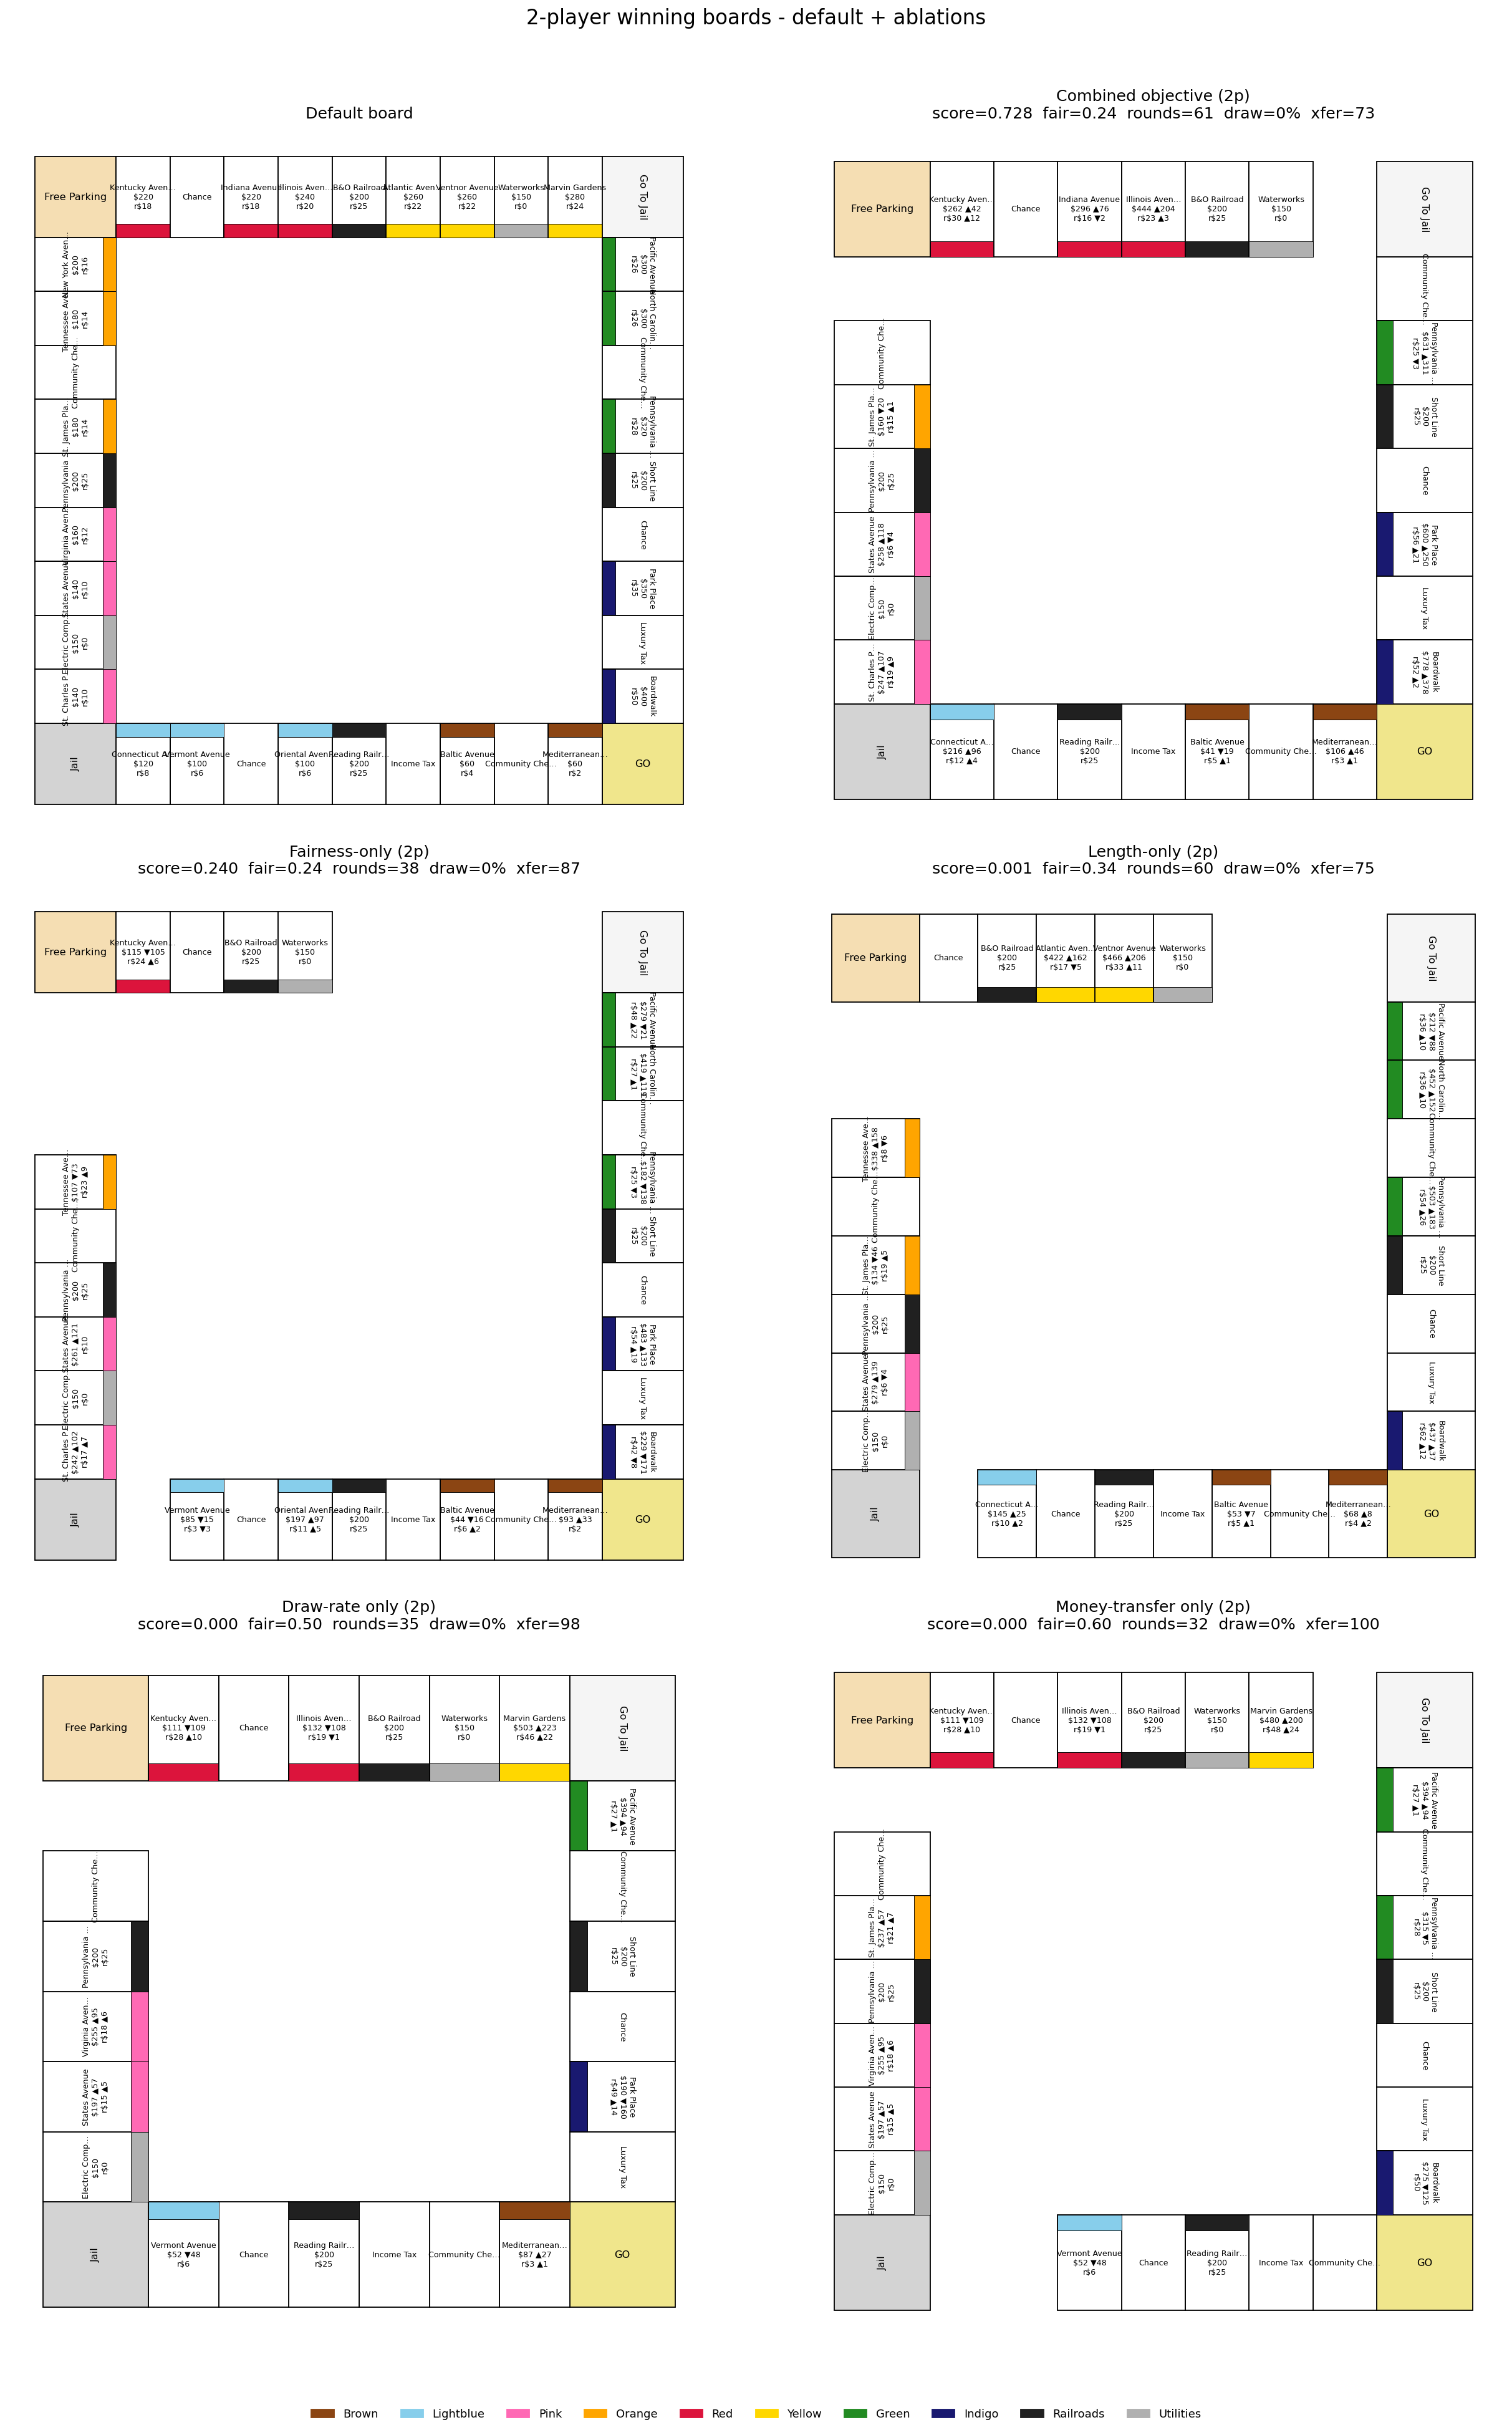
\includegraphics[width=\linewidth]{grid_2p_shrunk.png}
\caption{2-player ablation winners.}
\end{subfigure}
\begin{subfigure}{0.49\linewidth}
\centering
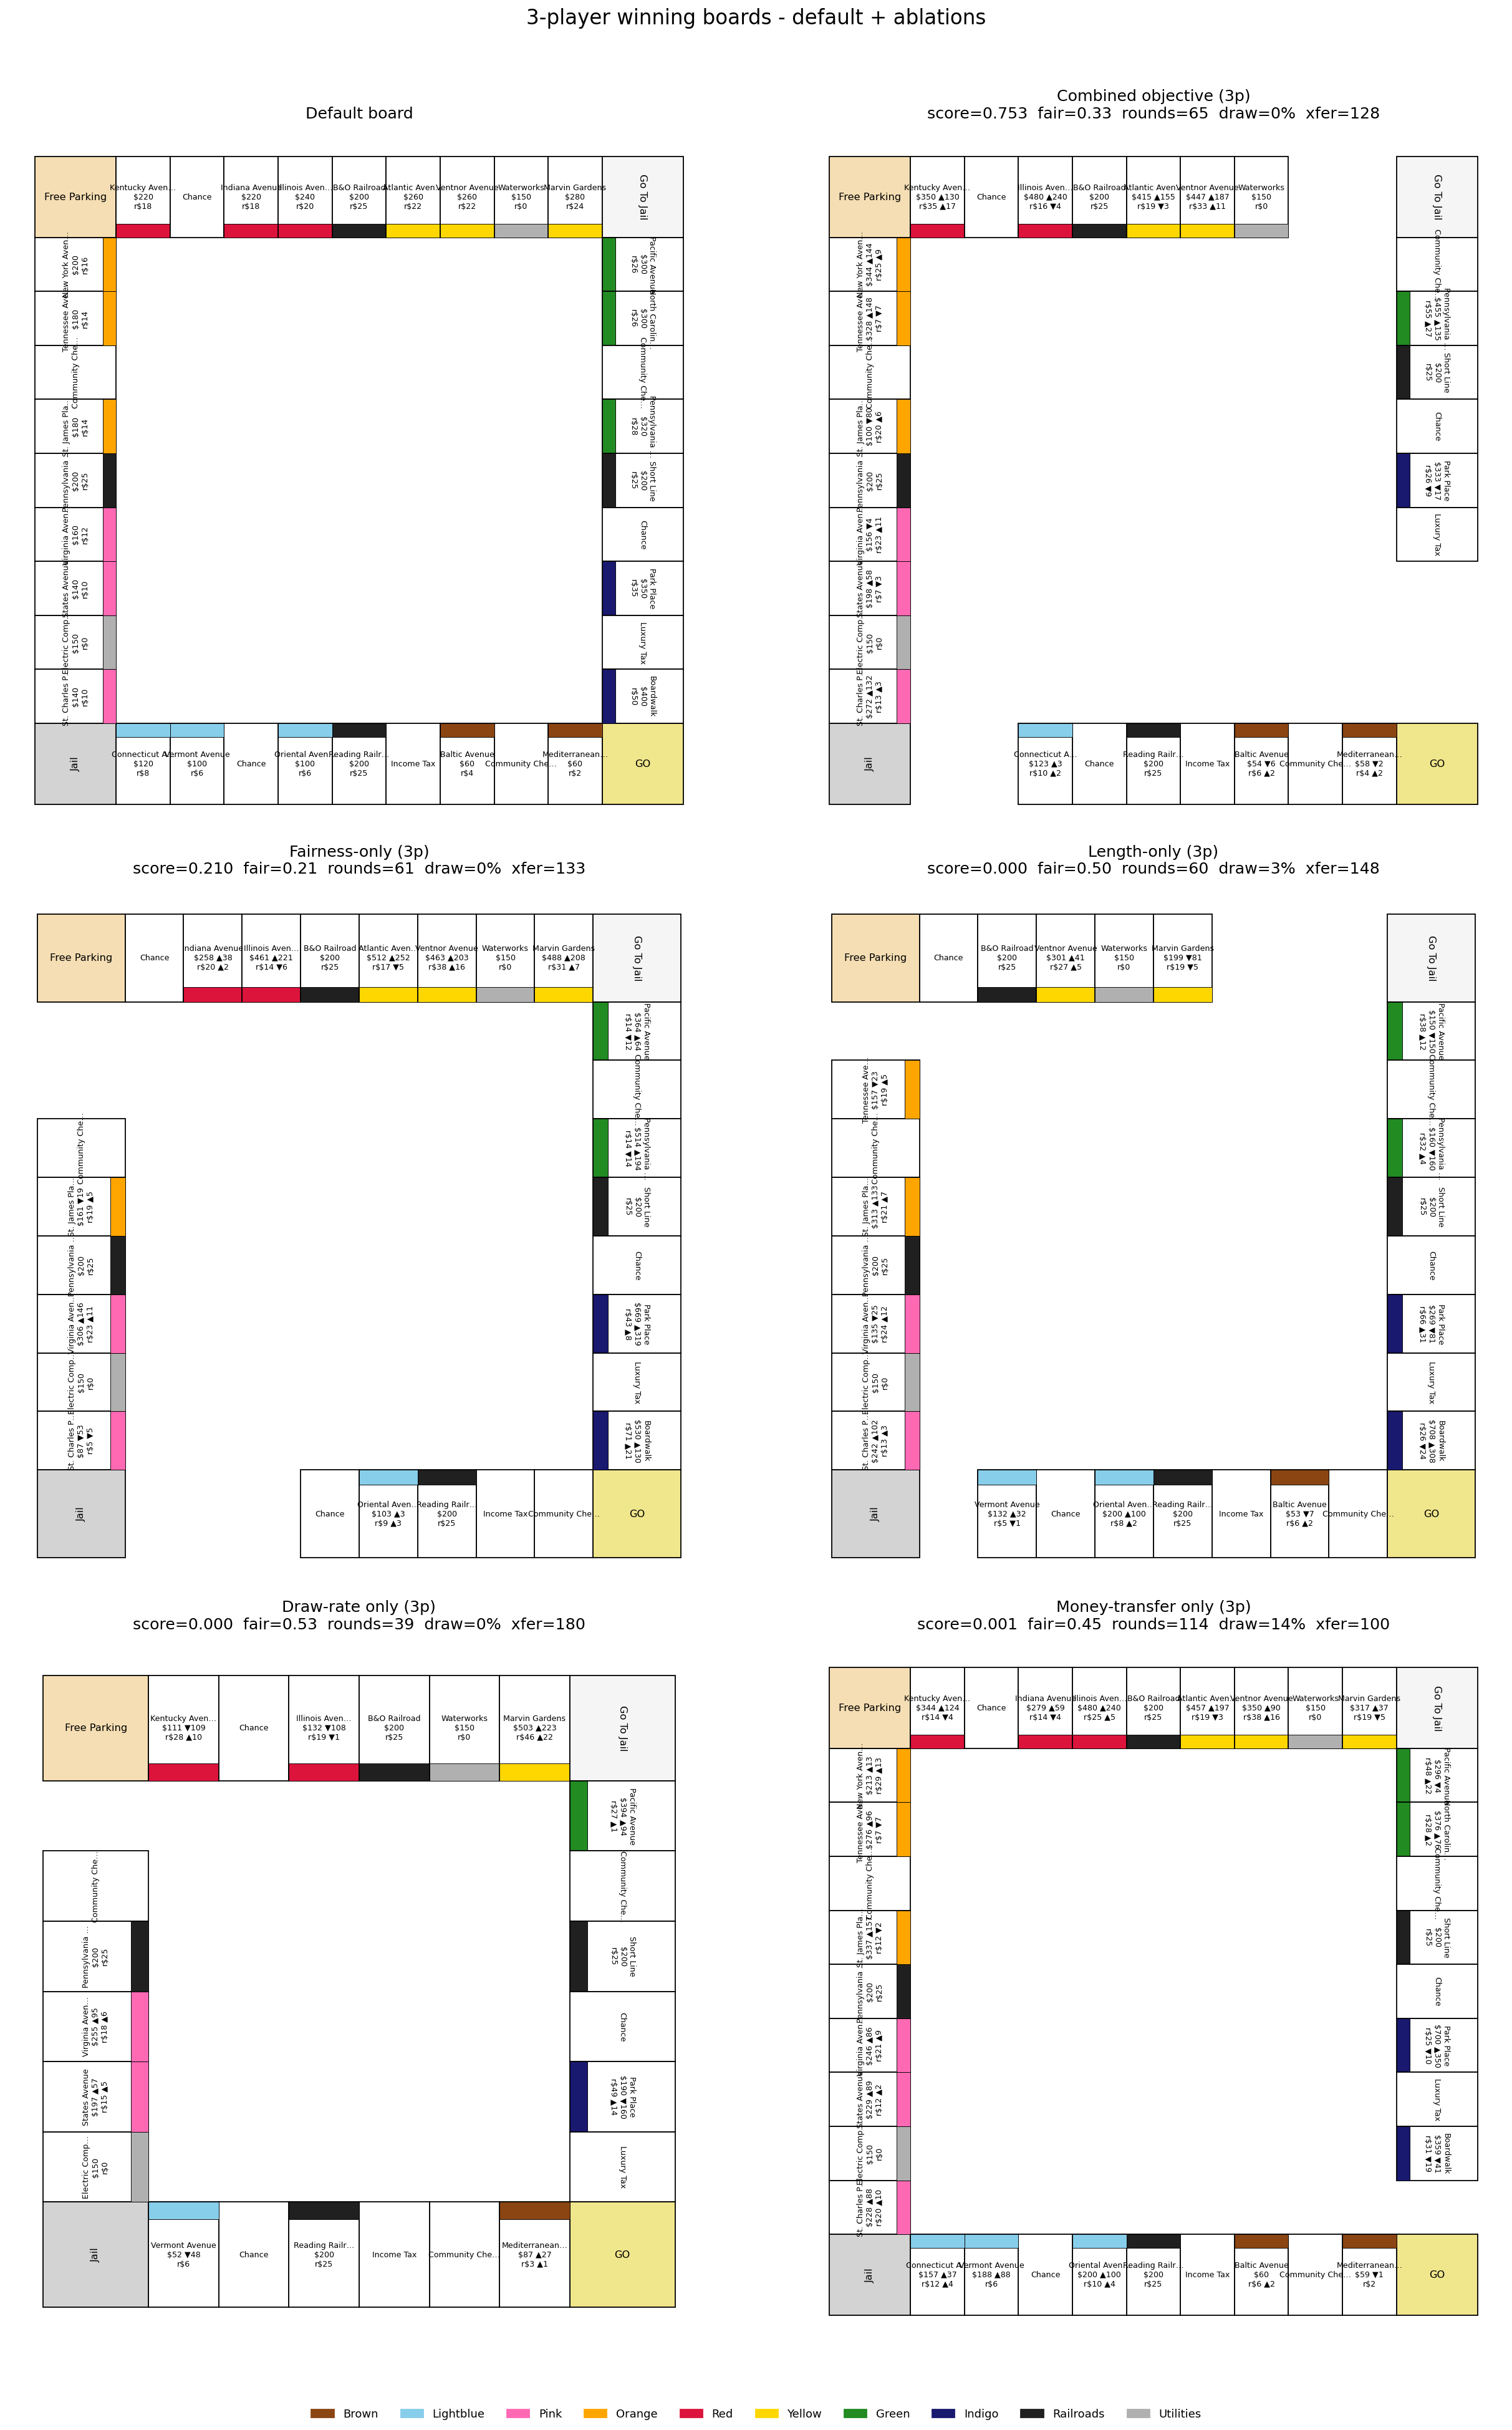
\includegraphics[width=\linewidth]{grid_3p_shrunk.png}
\caption{3-player ablation winners.}
\end{subfigure}
\caption{\textbf{Shrunk layout: winning boards rendered at their true
(post-shrinkage) cell count.} Each panel shows the default board (top-left)
alongside the winners of the four single-objective ablations (fairness,
length, draw-rate, money-transfer) and the combined-objective GA. The
optimised boards are \emph{physically smaller} than the default because
the design space includes a 22-bit keep-mask that lets the optimiser
delete colour-group properties entirely (not merely neutralise them).
Cell counts for each ablation's winner (2p): combined GA keeps 12/22
properties $\to$ 30 cells; fair-only 13/22 $\to$ 31; length-only 12/22
$\to$ 30; draw-only 9/22 $\to$ 27; money-only 10/22 $\to$ 28. All
intermediate cells are sized consistently so shorter boards produce
visibly smaller squares. This rendering foregrounds the \emph{pacing}
consequence of the design: optimiser-preferred boards take fewer turns
to complete a lap, accelerating salary accumulation and shortening
games, which is the mechanism behind the 30-40\% round-count reductions
reported in Table~\ref{tab:cross}.}
\label{fig:boards_shrunk}
\end{figure}

\begin{figure}[h]
\centering
\begin{subfigure}{0.49\linewidth}
\centering
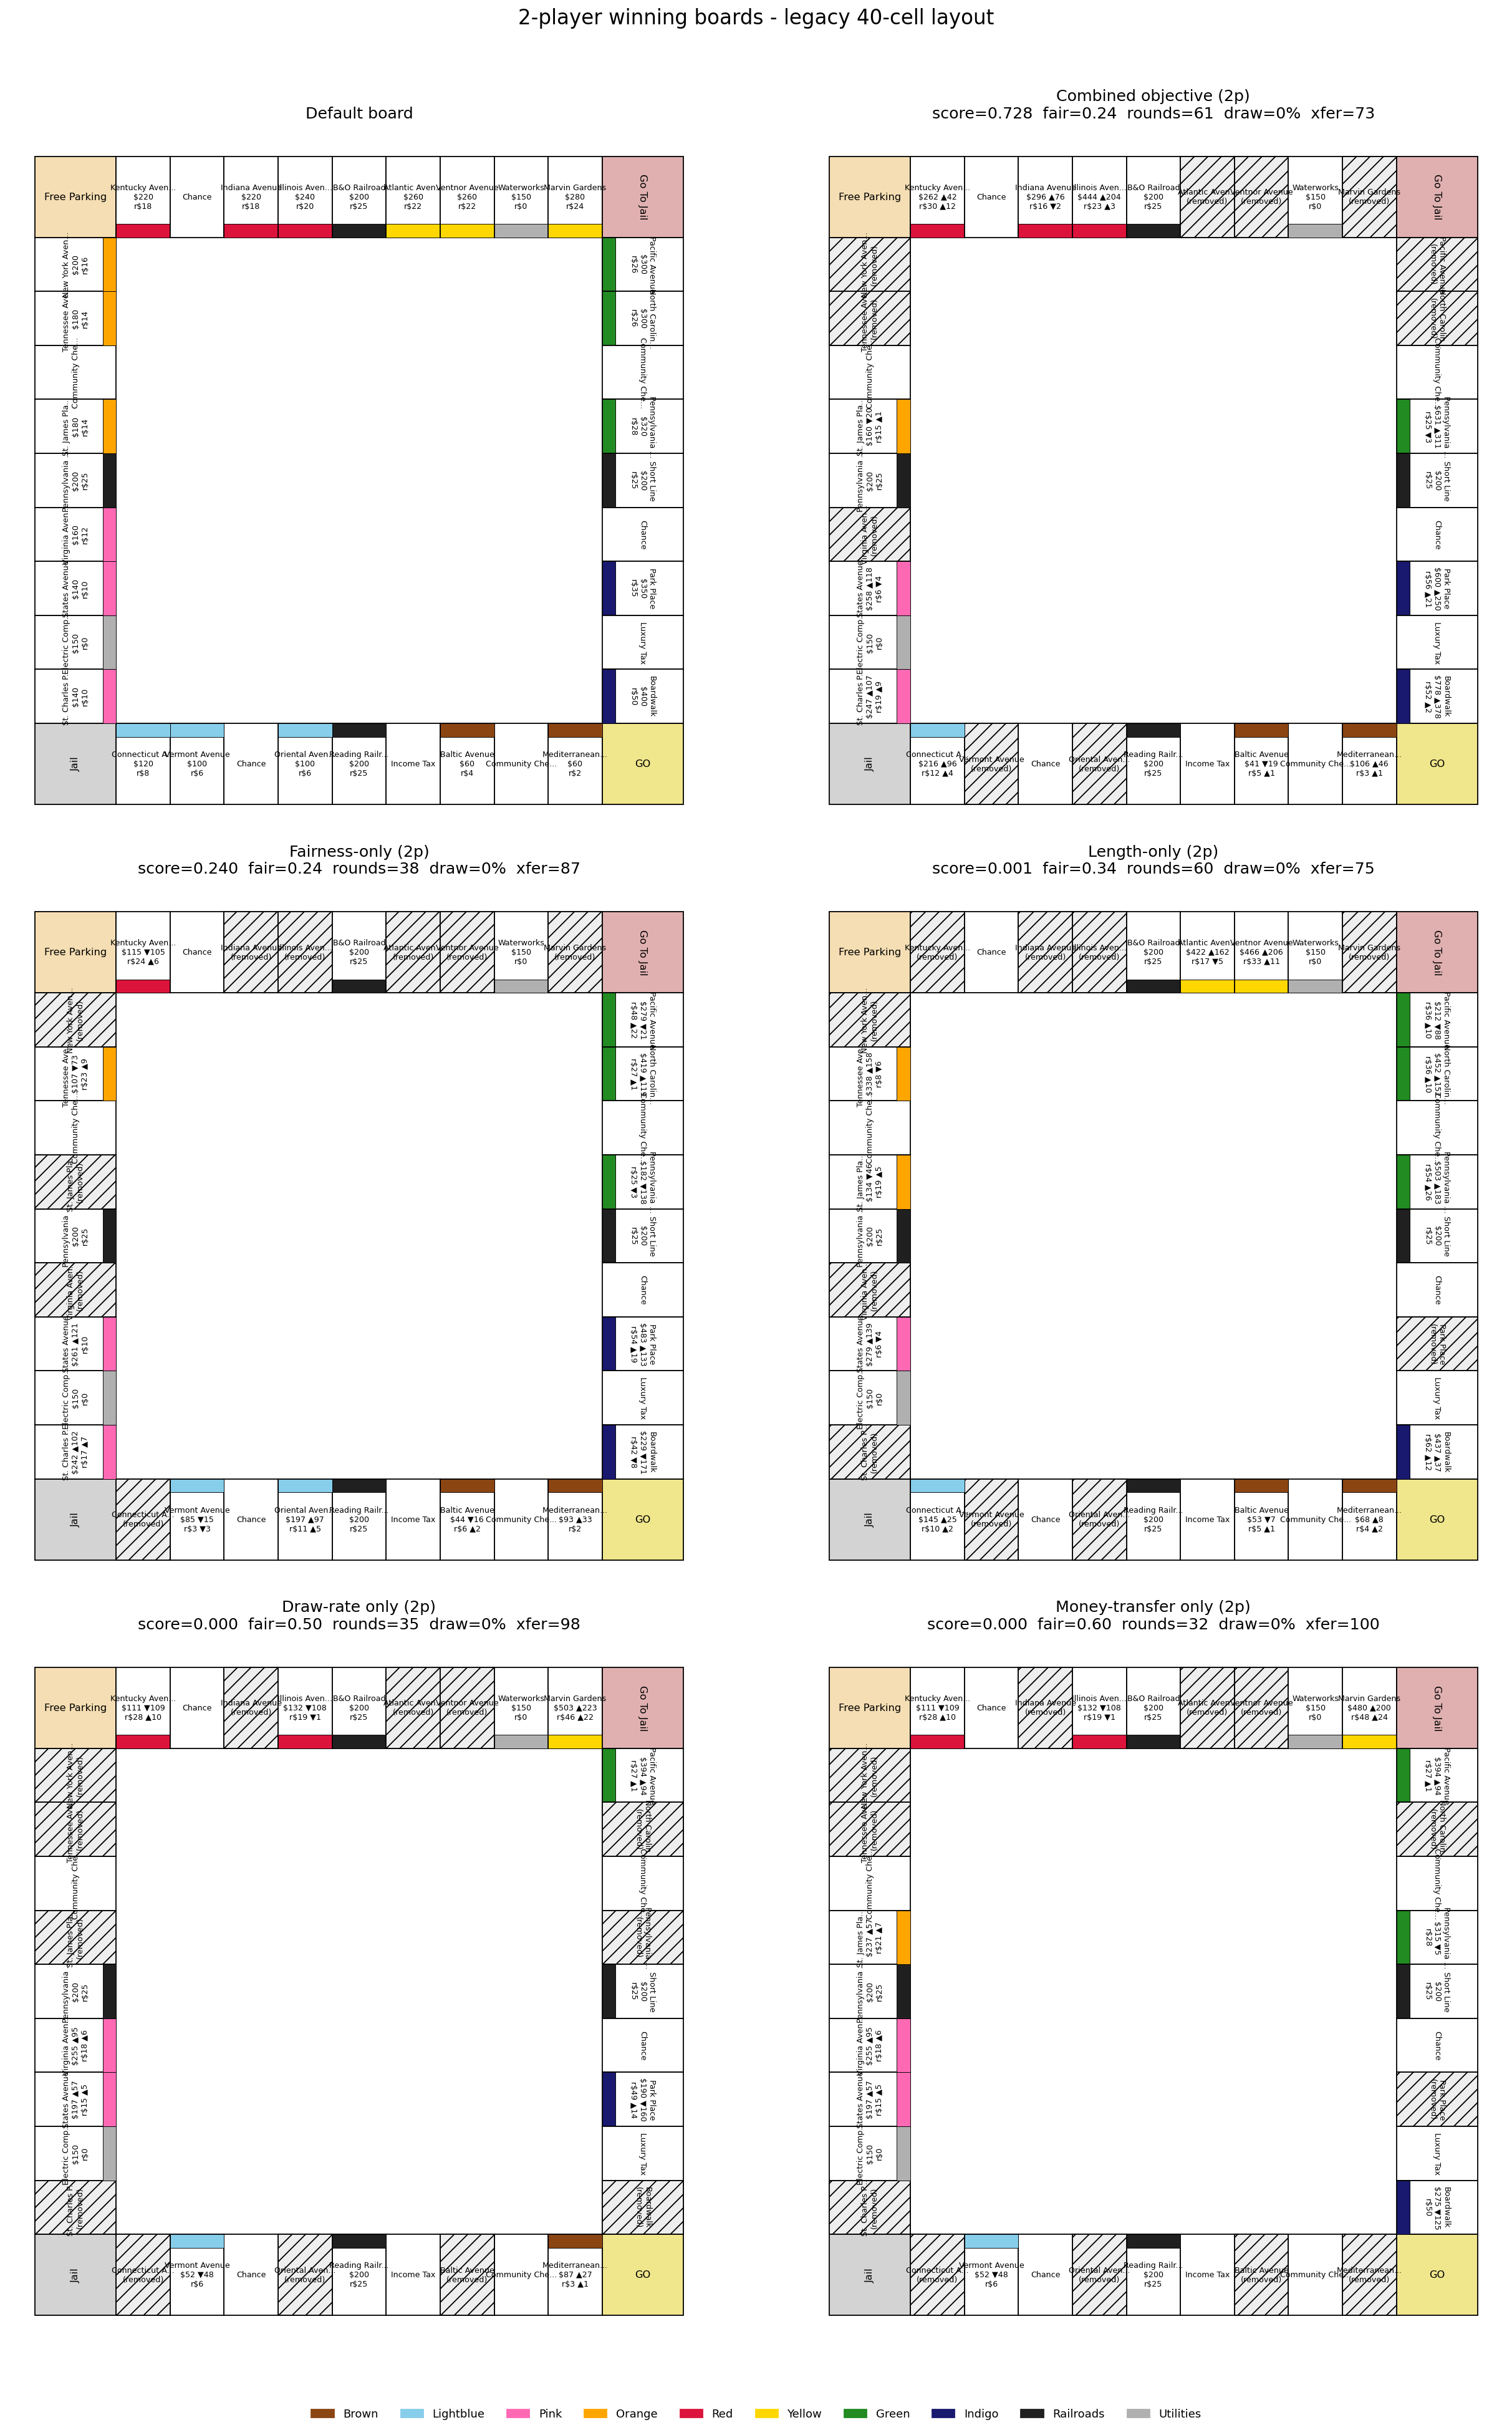
\includegraphics[width=\linewidth]{grid_2p_legacy.png}
\caption{2-player ablation winners.}
\end{subfigure}
\begin{subfigure}{0.49\linewidth}
\centering
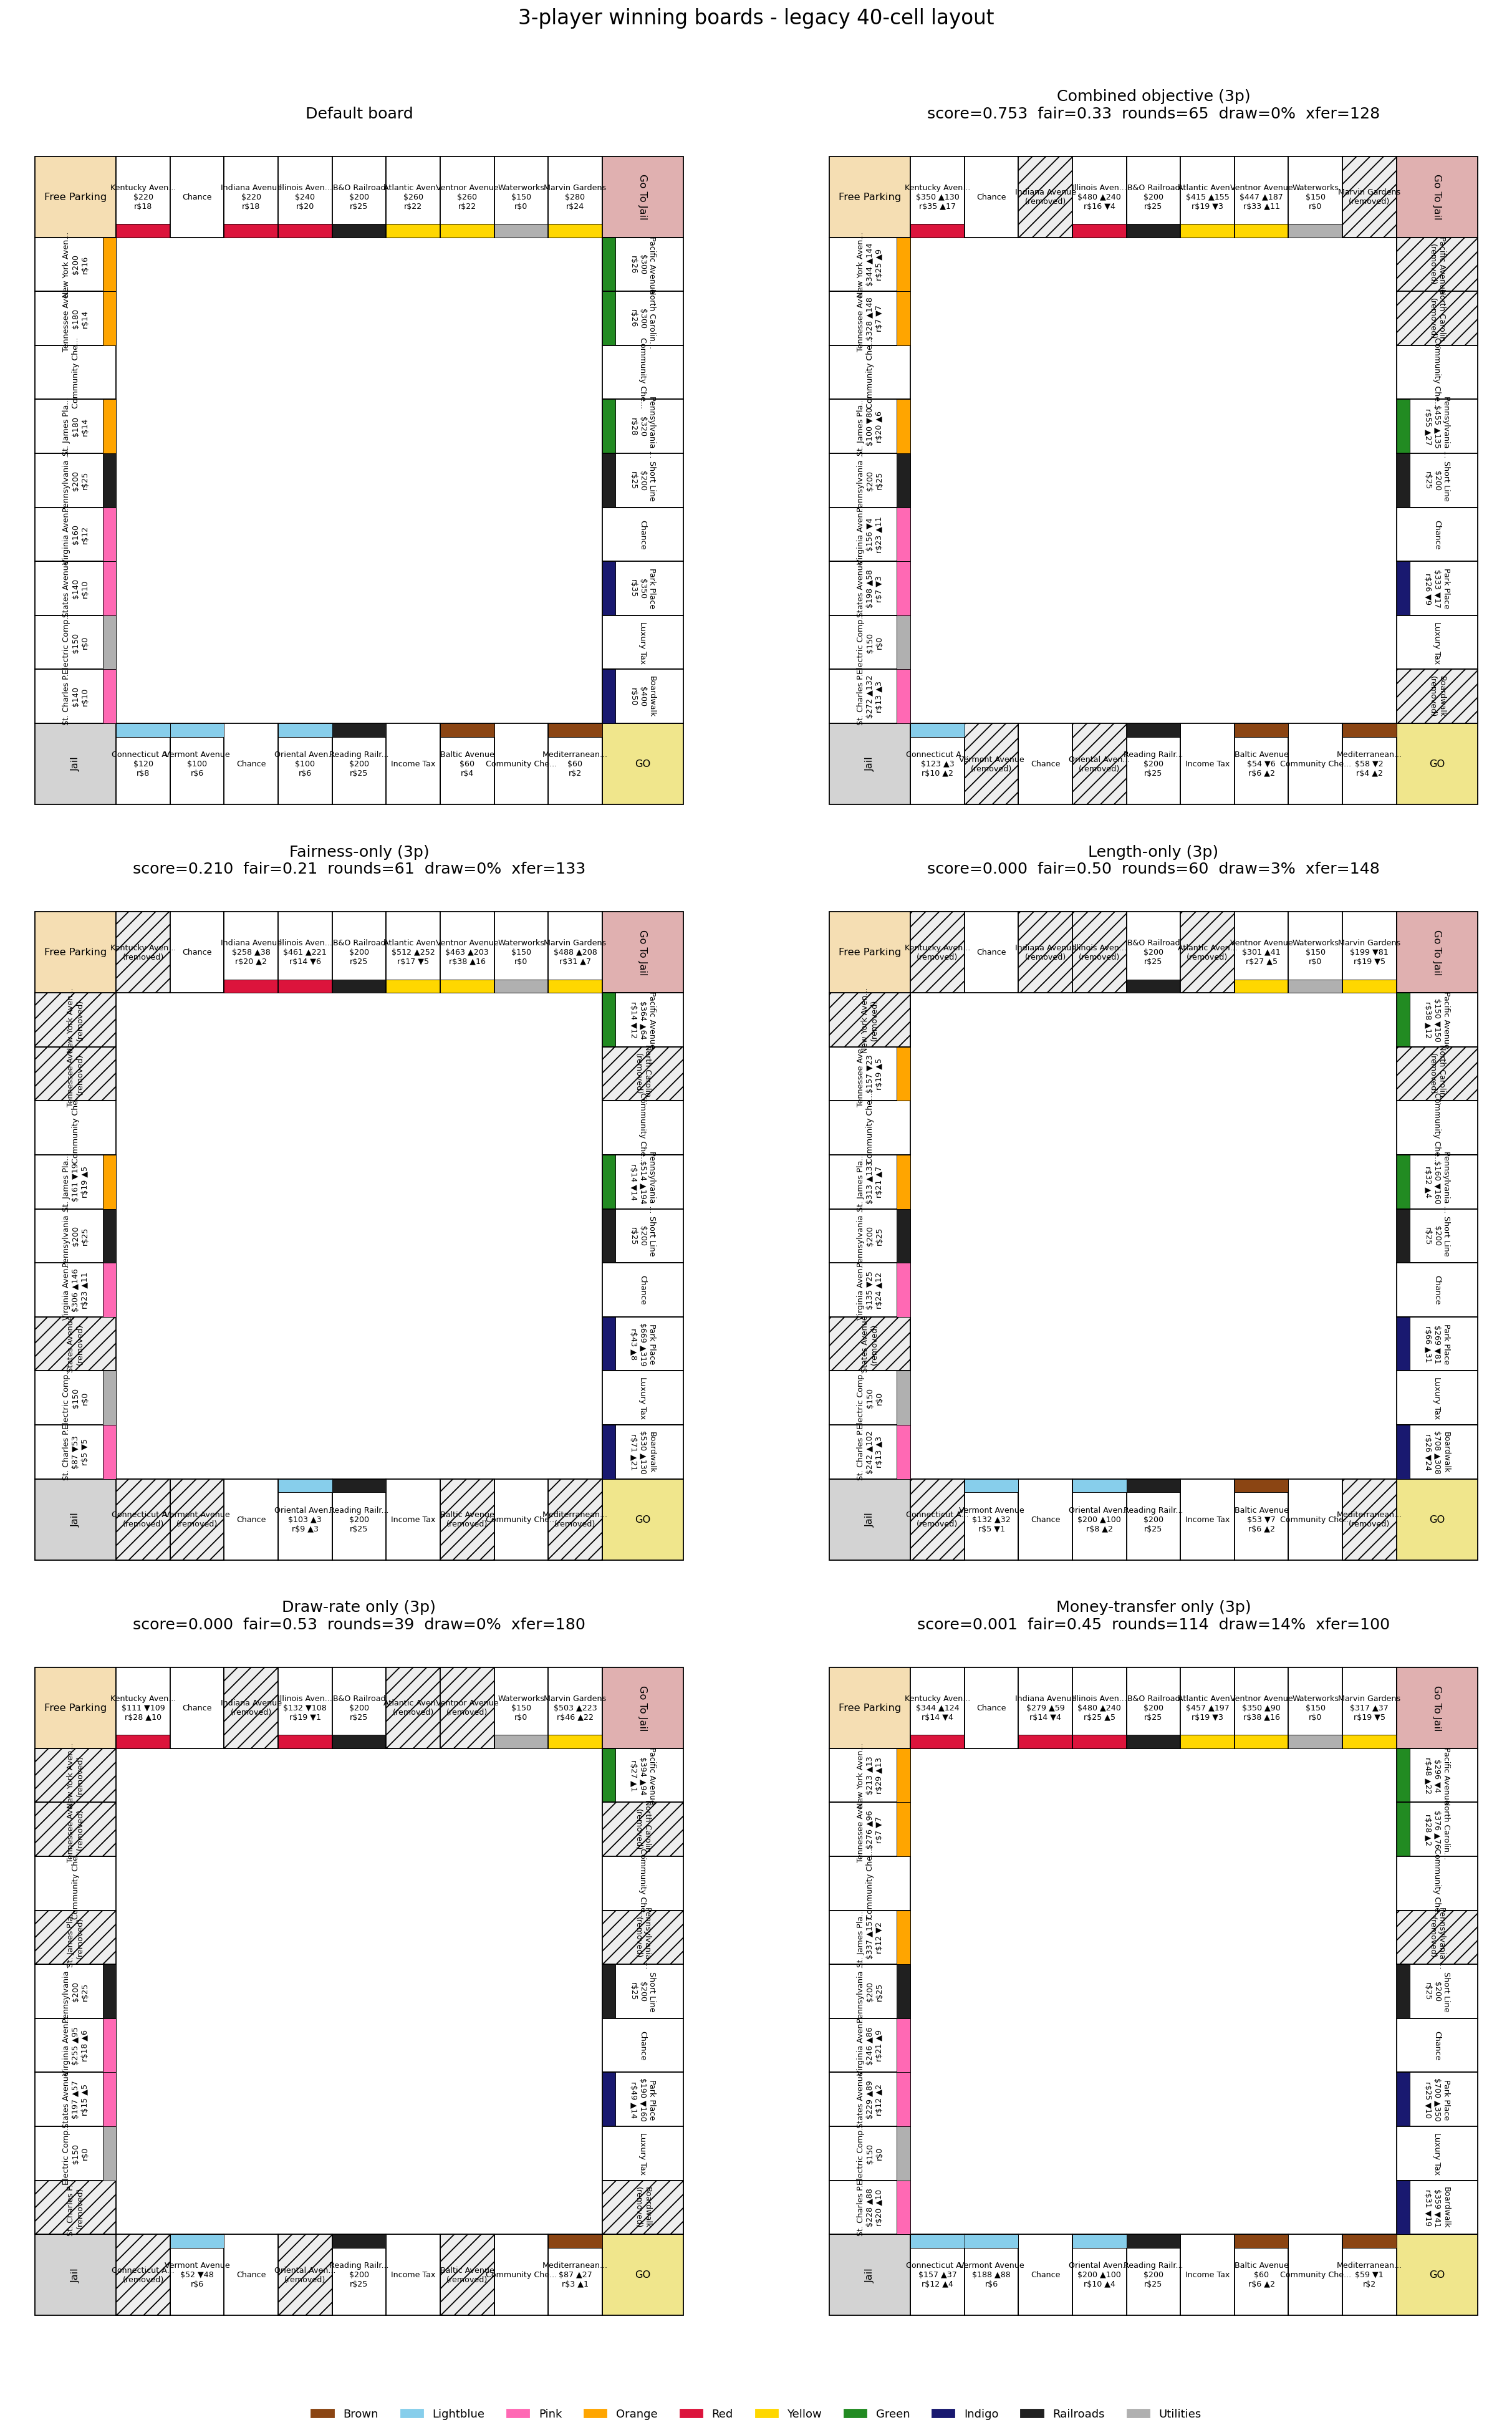
\includegraphics[width=\linewidth]{grid_3p_legacy.png}
\caption{3-player ablation winners.}
\end{subfigure}
\caption{\textbf{Legacy layout: same designs rendered on the canonical
40-cell Monopoly board for direct positional comparison.} Identical
data to Figure~\ref{fig:boards_shrunk}, but the removed properties are
shown in-place as hatched ``(removed)'' cells rather than being deleted
from the board. This rendering preserves the canonical perimeter
(corners at indices 0/10/20/30; all colour-group positions at their
default Monopoly slots) so a reader can see \emph{which} specific
properties each objective chose to drop. Two patterns are visible:
(i) fairness-oriented objectives (fair, draw) aggressively remove
multiple colour groups from expensive-rent positions; (ii) the
money-only 3p winner is near-full-length because 3-player default
already saturates inter-player transfer, leaving little room for
shrinkage to help. The ▲/▼ annotations on surviving properties show
cost/rent multiplier deltas against the default board. Taken together,
the two figures decouple the two axes of the design: \emph{which}
properties are present (Fig.~\ref{fig:boards_legacy}) and \emph{how
long the lap is} (Fig.~\ref{fig:boards_shrunk}).}
\label{fig:boards_legacy}
\end{figure}

\subsection{Non-obvious findings vs.\ sanity checks}\label{sec:nonobvious}

It is worth distinguishing the findings the agent loop \emph{surfaced}
from the findings that fall out of the design space by construction.
Several of the headline numbers are the latter: shorter boards produce
shorter games (because dice rolls wrap mod $40-k$, so the lap is
shorter), zero draws are achievable (because the optimiser can drop
properties until no all-rich stalemate is possible), and so on. These
are sanity checks that the optimiser is not broken; they are
\emph{not} insights about Monopoly that a designer could not have
predicted before running the sweep.

Three findings genuinely qualify as non-obvious insights surfaced by
the agent loop:

\begin{enumerate}[leftmargin=1.2em,itemsep=2pt]
\item \textbf{Environment design moves strategy-pair-level fairness.}
The mean per-pair $|W{-}0.5|$ across the 30$\times$30 strategy matrix
drops from $0.21$ on the default board to $0.17$ on the GA-2p winner
(Section~\ref{sec:heatmap}). A natural prior is that strategy-skill
asymmetries are properties of the strategies, not the board, and that
environment changes should leave the matrix structure roughly fixed.
The optimiser falsified that prior: changing per-property cost/rent
multipliers and the keep-mask redistributed which strategy archetypes
beat which others, not just the global pacing.

\item \textbf{The GA-3p winner is universally the best 2p design.}
Cross-evaluation at $n{=}1000$ shows the GA-3p board scores $0.954$ on
the 2p harness, \emph{better} than the GA-2p board's own 2p score of
$0.998$ (Table~\ref{tab:cross}). The 3p optimisation incidentally
exercises more strategy interactions (every game has 3 active
participants), pressure-testing the design more thoroughly than 2p
optimisation does. A designer optimising for 2p only would have missed
this; the cross-evaluation surfaced it.

\item \textbf{Default 3-player Monopoly already saturates inter-player
cash flow.} The money-only ablation in 3p barely deviates from the
default board (kept $20$ of $22$ properties, score $\approx 0$ at
$\overline{T}=100.2$) because the default 3p board already produces
$\overline{T}=98.2$/round, $\$2$ short of target. The same ablation in
2p must aggressively shrink the board (kept 9/22 properties, $\approx 30$
rounds/game) to lift transfer from $50$ to the $100$ target. This is a
real \emph{design} insight: in 2p Monopoly the transfer rate is the
hardest objective to satisfy without breaking other dimensions; in 3p
it is essentially free. A designer would otherwise have to discover
this by hand.
\end{enumerate}

These three are precisely the kinds of findings that make the
beta-testing loop worth building rather than running each design change
by hand: the loop surfaces structural patterns that intuition would not
have predicted, but that hold up under scrutiny once seen.

\section{Generalisation: lessons for multi-agent system design}\label{sec:gen}

The framework here transfers to any multi-agent system whose designer can
parameterise the environment and evaluate it against a population of
agents. We extract eight transferable principles, supported by specific
findings from the Monopoly study.

\paragraph{What the agent loop can be trusted for.} Before listing the
principles it is worth being explicit about the scope of trust an
automated agent-based beta-testing loop can offer. Agent metrics are
trustworthy for the \emph{direction} and \emph{relative magnitude} of a
design change: ``board X has shorter games than board Y'', ``ablation Z
disproportionately affects fairness''. They are \emph{not} trustworthy as
absolute predictors of human-experienced outcomes: ``humans will
produce a $0.24$ mean fairness on this board'' is overclaiming. Every
claim below should be read with this calibration in mind, and is the
reason Section~\ref{sec:validation} commits to a real-human validation
phase rather than declaring victory on the agent-internal scoreboard.

\begin{enumerate}[leftmargin=1.2em,itemsep=2pt]
\item \textbf{Strategy-pool diversity beats single-oracle evaluation.}
We initially planned to train one RL agent and optimise the board against
it. We instead curated 30 diverse rule-based strategies and optimised for
robustness across the pool. \emph{Lesson}: when you cannot enumerate
rational behaviours, sampling the strategy space and aggregating gives a
more honest quality estimate than optimising against any single agent.

\item \textbf{Robust aggregation as the objective.} Our objective combines
\emph{mean} fairness with a \emph{worst-case} term ($w_{\text{fmax}}$).
\emph{Lesson}: in any multi-agent system (auction, recommendation,
matchmaking), adding a worst-case term forces the optimiser to treat the
tail as a hard constraint, not noise.

\item \textbf{Per-objective ablations expose trade-offs.} Each ablation
drove its target to its lower bound but degraded a different objective
(Table~\ref{tab:ablation}). \emph{Lesson}: in multi-objective design,
the only way to know a composite objective is well-balanced is to run
each component isolated and compare.

\item \textbf{Some asymmetries are agent-level, not environment-level.}
\textsl{RailroadKing} loses 0\%/100\% to multiple aggressive buyers on
\emph{any} board our space can produce. \emph{Lesson}: when a designer
sees an unfixable system-level asymmetry, the budget should redirect to
agent-level intervention (training, education, matchmaking) rather than
more environment iterations.

\item \textbf{Evaluate under counterfactual deployment regimes.} The
GA-3p winner is also the best 2p design; the GA-2p winner is competitive
but not best at 3p. \emph{Lesson}: cross-evaluation across deployment
regimes is cheap and routinely catches over-fits to the optimisation
context.

\item \textbf{Behavioural interactivity as a first-class metric.}
Money-transfer rate measures inter-agent state flow per turn, an
interactivity proxy independent of the headline win signal. We found 2p
default \emph{under-saturates} this dimension (50/round vs.\ target 100)
while 3p default already saturates (98/round). \emph{Lesson}: in
intentionally interactive systems, an interactivity proxy belongs in
the objective alongside outcome metrics.

\item \textbf{Variance-reduction discipline beats more samples.} Identical
$(\text{seeds},\text{matchups})$ across candidates makes an unchanged
design produce byte-identical metrics. The GA's signal was visible at
$n{=}100$ games per candidate; without shared random numbers we would
need $\sim 1000$. \emph{Lesson}: common random numbers (CRN) are
under-used in multi-agent evaluation pipelines.

\item \textbf{Problem framing dominates optimiser choice.} The GA beats
random search by 16--17\%, not orders of magnitude. The big lift came
from defining the right strategy pool, the right objective, and the
right evaluation protocol. \emph{Lesson}: in system design, problem
formulation is almost always the bottleneck, not optimiser cleverness.
\end{enumerate}

\section{Limitations}

\textbf{No human-validation evidence yet.} Every result reported in
Section~\ref{sec:eval} is internal to the agent loop: agents played the
optimised boards and produced metrics that the optimiser itself selected
for. We have not yet observed humans playing these boards. The central
project claim (agent feedback is directionally predictive of real
play) is therefore not falsified \emph{or} confirmed by the current
evidence. Section~\ref{sec:validation} commits to a concrete plan that
closes this gap; everything below is contingent on its results.
\textbf{Strategy pool representativeness.} If real users behave outside our
17-dim parametric space, an optimised board may misfit them. Mitigation:
sample more or learn the strategy distribution from logs.
\textbf{Objective decomposability.} Real-world goals like ``fun'' or
``engagement'' may not decompose into the 4--5 metrics we use. The
framework supports adding new metrics; the choice is the designer's.
\textbf{Optimisation-set overfit.} The $n{=}100$ optimisation budget
overfits its specific seed/matchup choice by $\approx 0.17$ score points
relative to $n{=}1000$ evaluation. The relative ranking of designs is
preserved.
\textbf{Structural shrinkage and the canonical perimeter.} Properties
removed by the keep-mask are deleted from the board, shortening it from
40 cells; we route Chance / Community Chest cards that target specific
named properties through a name-based lookup that gracefully no-ops when
the target has been removed. This is faithful but means the dice-roll
distribution shifts when the board shrinks, conflating the
``properties present'' axis with the ``board length'' axis. A purer
ablation that decouples the two is left for future work.

\section{Validation plan}\label{sec:validation}

The central claim of this project (agent feedback is directionally
predictive of human play) is not yet supported by direct evidence. This
section commits to a three-phase validation plan whose pre-declared
methodology, statistics, and falsification criteria collectively
operationalise the claim. The plan is structured so that each phase
generates a different kind of evidence about \emph{when} agent feedback
is decision-useful and when it is not.

\subsection{Phase A: simplified-board sanity check}

Before running humans on the full board, we run the same pipeline on a
deliberately simplified $4{\times}4$ ($16$-cell) variant. The simplified
board has:
\begin{itemize}[leftmargin=1.2em,itemsep=0pt]
\item 4 corner cells (GO, Jail, Free Parking, Go-To-Jail) at the same
relative positions as the canonical board.
\item 4 colour-group properties (one short Brown, one short Lightblue,
one short Pink, one short Orange).
\item 2 Chance / Community Chest cells.
\item 2 Tax / Special cells.
\end{itemize}
This is small enough that a human game completes in 5--10 minutes and a
single design knob has a tractable, isolatable effect. The purpose of
Phase A is to test the \emph{plumbing}: does our agent setting produce
the same sign of effect on a simplified board where the answer is
intuitively predictable, before we commit time to the full board?

\paragraph{Pre-declared design knobs.} We will vary three knobs one at a
time and record the agent-predicted effect, then verify in human play:
(i) salary doubled vs.\ default (expect: shorter games, fewer draws);
(ii) one colour-group property removed vs.\ default (expect:
fewer monopolies, more draws); (iii) rent on the most expensive group
doubled vs.\ default (expect: higher win-rate spread, more bankruptcies).

\subsection{Phase B: human playtest}

After Phase A passes the sanity check, we recruit $3$--$5$ human
playtesters and run $5$--$10$ games per board on the full canonical
board, comparing the default to one or two GA-optimised winners. We
collect per-game data using the same script as the agent simulator:
winner identity, round count, bankruptcy log, total inter-player cash
transfer. We also collect $5$-point Likert ratings from each tester
after each game on perceived fairness, perceived length, and engagement.

\paragraph{Falsification criterion.} The agent loop is judged
\emph{decision-useful} if at least two of the three pre-declared knobs
in Phase A produce the same sign of effect in human play, AND if the
GA-optimised board's mean human-rated fairness exceeds the default
board's mean human-rated fairness on a paired-sample $t$-test at
$p<0.1$. The agent loop is judged \emph{not decision-useful} if humans
report no perceptible difference between the boards, or if the sign of
the effect contradicts the agent's prediction on $\geq 2$ of $3$ knobs.

\subsection{Phase C: LLM-agent cross-check}

A third independent signal is provided by an LLM-based player
(\texttt{LLMPlayer}, registered in our codebase using a lightweight
local Qwen2.5-0.5B-Instruct model). The LLM is given the current game
state (cash, owned properties, board occupancy, colour-group
completion) and asked at each decision point to choose buy/no-buy or
build/no-build. We run the same boards from Phase B with the LLM in
place of the rule-based agents and compare the same statistics.

\paragraph{Why a third signal.} The rule-based pool, the LLM, and the
human cohort exhibit fundamentally different reasoning styles. If all
three agree on the direction of an effect, we have very strong evidence
that the design change is real. If they disagree, the disagreement
itself is informative: it tells us which agent class the designer can
trust on which dimension. Specifically: rule-based agents are likely
most reliable on \emph{quantitative} effects (game length, transfer
rate); LLMs are likely more reliable on \emph{strategic/contextual}
effects (which strategy archetype actually wins under which board);
humans are the only signal on \emph{subjective} effects (perceived
fairness, fun).

\subsection{Pre-declared statistics across all three phases}

\begin{table}[h]
\centering
\small
\begin{tabular}{lp{6cm}}
\toprule
Statistic & Operationalisation \\
\midrule
mean game length     & turns until $\leq 1$ non-bankrupt player remains, or until truncation \\
std game length      & standard deviation of the above across the recorded sessions \\
draw rate            & fraction of games hitting the 200-turn truncation cap (rule-based / LLM) or hitting a $90$-minute real-time cap (human) \\
per-archetype win rate & rule-based: counted by strategy name; LLM: model is single-archetype, but seat order rotates; human: testers self-classify into one of the named archetypes pre-game \\
time to first monopoly & turns until any player completes any colour group \\
mean rent paid       & total rent paid by each player divided by games played, averaged \\
bankruptcies/game    & count of \texttt{is\_bankrupt} flags at game end \\
mean transfer/round  & rule-based / LLM: as in Section~\ref{sec:problem}; human: self-recorded on a printed score sheet at game end \\
\bottomrule
\end{tabular}
\caption{\textbf{Pre-declared summary statistics for cross-source
comparison.} The same eight statistics will be computed from each of
the three sources (rule-based agents, LLM agent, humans) on each board
in the validation phases. Pre-committing this list before the human
playtest is what makes the eventual cross-comparison legitimate, rather
than a post-hoc selection of whatever signal happened to look clean.}
\label{tab:pre_decl_stats}
\end{table}

\subsection{What success looks like}

We do not need agents to predict human numbers. We need agents to
predict the \emph{ranking} of designs along each dimension we care
about. Concretely, success means: when the agent loop says ``board $A$
has shorter games than board $B$'' or ``board $A$ is fairer than board
$B$'', the human play data should produce the same ranking, even if the
absolute numbers differ. If this rank-correlation holds, the agent
loop is exactly the kind of beta-testing tool a designer wants: it
lets them throw 100 candidate designs at a fast simulator, pick the 1
or 2 that look best on the dimensions of interest, and trust that those
designs will generally play better with humans too.

\section{Conclusion}

We built a closed-loop game-design optimiser for Monopoly that uses a
diverse parametric strategy pool as the evaluator and improves a
combined fairness/length/draw/interactivity score by 32\%--46\%
($n{=}1000$) on both 2-player and 3-player versions, beating random
search by 16--17\% at equal evaluation budget. The framework, and its
eight extracted MAS principles, generalises to environment design
problems where (i) the environment can be parameterised, (ii) a
diverse agent population can be assembled, and (iii) evaluation is cheap
relative to the search budget.

\paragraph{Reproducibility.} All experiments live under
\texttt{monopoly/logs/optimizer/} as JSONL run logs and JSON summaries.
Every figure and table number can be regenerated by re-running
\texttt{scripts/optimize\_board.py}, \texttt{scripts/cross\_eval.py},
\texttt{scripts/strategy\_heatmap.py}, and \texttt{scripts/report\_runs.py}
with the seeds recorded in each run's \texttt{.meta.json}.

\appendix

\section{Implementation details}\label{app:impl}

\paragraph{Codebase organisation.} The optimiser lives under
\texttt{monopoly/optimizer/} as a self-contained package: \texttt{simulate.py}
(per-game stat collection), \texttt{design\_space.py} (vector~$\leftrightarrow$
\texttt{GameConfig}), \texttt{objectives.py} (pure functions over game
results), \texttt{strategy\_pool.py} (strategy definitions + evaluation
matchup sampler), and \texttt{search.py} (random search + GA). CLI drivers
live under \texttt{monopoly/scripts/} as one script per user-facing action
(\texttt{optimize\_board.py}, \texttt{cross\_eval.py},
\texttt{strategy\_heatmap.py}, \texttt{report\_runs.py},
\texttt{render\_board.py}, \texttt{render\_all\_boards.py}, and two legacy
variants that preserve the canonical 40-cell renderer).

\paragraph{Simulator instrumentation.} We reuse the upstream Monopoly core
game loop (\texttt{monopoly/core/game.py}) unchanged except for making
board landmark positions (GO, Jail, Go-to-Jail, Free Parking) resolve
dynamically via \texttt{Board.jail\_index} etc., so the engine supports
shorter-than-40-cell boards correctly. Chance and Community-Chest cards
that target specific named cells (``Advance to Boardwalk'',
``Advance to Illinois Avenue'', ``Advance to the nearest Railroad''
etc.) look their targets up by name at runtime, gracefully no-oping
when the target cell has been removed by the design mask. Per-game
stats that the core loop does not return (winner, rounds, bankruptcy
status, total inter-player cash transfer) are captured by a
context-manager monkey-patch of \texttt{Player.pay\_money} that tallies
cash deltas from one \texttt{Player} recipient to another; bank
payments (salary, tax, fines) are excluded by design, because the
``interactivity'' metric should only count agent--agent flow. An
additional context-manager caps
\texttt{Player.do\_a\_two\_way\_trade} calls to $5$ per (player, turn)
pair to break an unbounded \texttt{while} loop in the upstream
trade-negotiation code; in pathological strategy pairings two
aggressive traders could otherwise cycle forever, stalling the entire
optimisation sweep.

\paragraph{Design space: encoding and clipping.} The design vector is
$66$-dimensional: $22$ continuous cost multipliers $\in[0.5,2.0]$, $22$
continuous rent multipliers $\in[0.5,2.0]$, and $22$ binary keep-bits
(the mask). The decoder applies cost multipliers to \texttt{cost\_base}
and \texttt{cost\_house} and rent multipliers to \texttt{rent\_base}
and every element of the \texttt{rent\_house} tuple. Integer rounding
is clipped to $\geq 1$ so no property becomes literally free. Masked-off
properties are \emph{deleted} from the \texttt{cells} list, so the board
becomes $40 - \text{drop-count}$ cells long; the game-loop instrumentation
above handles this correctly. A soft constraint prevents degenerate
boards: if a candidate has fewer than MIN\_KEPT$=8$ mask bits set, the
clip routine flips off-bits on until the floor is reached. Crucially,
\emph{this popcount repair is seeded deterministically from the SHA-256
digest of the vector itself} rather than Python's built-in
\texttt{hash()}, because the latter is randomised per-process via
\texttt{PYTHONHASHSEED} and would destroy the reproducibility guarantee
across runs. An earlier implementation used \texttt{hash()} and produced
$\pm 0.03$ score drift between fresh Python processes on identical
seeds; switching to SHA-256 restored byte-identical reruns.

\paragraph{Genetic algorithm.} Population $20$, $10$ generations (unless
otherwise noted), elitism $2$. Selection is $k{=}3$ tournament; crossover
is uniform (each dim independently swapped from parent A or B with
$p=0.5$); mutation is Gaussian $\sigma{=}0.1$ on continuous dims applied
per-dim with $p=0.1$, bit-flip with $p=0.05$ on binary dims. The design
vector is clipped after every sample / crossover / mutation operation,
so feasibility is always preserved. Elitism reuses scores from the prior
generation rather than re-evaluating, which reduces compute by roughly
$10\%$ per run at no quality cost (the shared-random-numbers discipline
guarantees identical scores on reruns anyway).

\paragraph{Determinism and reproducibility.} The full pipeline is
reproducible by construction. The design-vector seed, the strategy-pool
seed, the evaluation-matchup seed, and the per-candidate game seeds are
all fixed via CLI arguments. Every run writes a
\texttt{<run\_name>.meta.json} alongside the \texttt{<run\_name>.jsonl}
history with all of these seeds plus the CLI args, so any reported
number can be regenerated from its meta file alone. Total compute for
the full paper is $\sim$165k simulated games across $12$ optimisation
runs, two $n{=}1000$ cross-evaluations, and two $30\times30$ heatmaps,
completing in $\sim$25--50 minutes of single-CPU wall-clock depending on
population/generation settings.

\section{Strategy space catalogue}\label{app:strategies}

\paragraph{Parameter specification.} Every agent in the pool is a
\texttt{ParametricPlayer} configured by a
\texttt{ParametricPlayerSettings} dataclass with $17$ fields
(Table~\ref{tab:paramspec}).

\begin{table}[h]
\centering
\small
\begin{tabular}{llp{8cm}}
\toprule
Field & Range / type & Meaning \\
\midrule
\texttt{unspendable\_cash}        & $[0, 1500]$, int   & Cash below which the player refuses to buy a property. \\
\texttt{build\_cash\_floor}       & $[0, 1500]$, int   & Cash below which the player refuses to build a house/hotel. \\
\texttt{trade\_max\_diff\_absolute} & $[0, 500]$, int  & Maximum $ difference in trade value the player will accept. \\
\texttt{trade\_max\_diff\_relative} & $[1.0, 5.0]$, float & Maximum ratio of trade values the player will accept. \\
\texttt{jail\_pay\_threshold}     & $[0, 1500]$, int   & Cash above which the player pays the \$50 fine to leave jail early. \\
\texttt{is\_willing\_to\_make\_trades} & boolean       & Whether the player initiates or accepts trades at all. \\
\texttt{aggressive\_build}        & boolean            & Build up to the cash floor every turn vs.\ only when cash is comfortable. \\
\texttt{buy\_utilities}           & boolean            & Whether the player buys Utilities when landing on them. \\
\texttt{buy\_railroads}           & boolean            & Whether the player buys Railroads when landing on them. \\
\texttt{ignore\_property\_groups} & subset of 8 colour groups & Colour groups the player refuses to buy, regardless of other conditions. \\
\bottomrule
\end{tabular}
\caption{\textbf{Parametric agent specification} ($17$ degrees of freedom:
$5$ continuous, $4$ boolean, $1$ bit-mask of size $8$). These fields
jointly determine every buying, building, trading, and jail-exit decision
the agent makes during a game. Defaults for unspecified fields are
inherited from \texttt{StandardPlayerSettings} in the upstream codebase.}
\label{tab:paramspec}
\end{table}

\paragraph{Named archetypes.} Ten strategies are hand-designed to span
behaviourally distinct regions of the parameter space. Their exact
parameter values are listed in Table~\ref{tab:archetypes}; rationales
follow the table.

\begin{table}[h]
\centering
\scriptsize
\begin{tabular}{lrrrrccccl}
\toprule
Name & cash & build & $t_{\text{abs}}$ & $t_{\text{rel}}$ & trades & aggr.\ build & util & rail & ignore groups \\
\midrule
AggressiveBuilder & 0    & 0    & 200 & 2.0 & F & T & T & T & --- \\
CashHoarder       & 1000 & 1200 & 200 & 2.0 & F & F & T & T & --- \\
Trader            & 300  & 400  & 400 & 3.5 & T & T & T & T & --- \\
RailroadKing      & 100  & 100  & 200 & 2.0 & F & T & F & T & all 8 colour groups \\
LowCostOnly       & 200  & 250  & 200 & 2.0 & T & T & T & T & Orange, Red, Yellow, Green, Indigo \\
HighCostOnly      & 400  & 500  & 200 & 2.0 & T & T & F & T & Brown, Lightblue, Pink \\
Balanced          & 300  & 350  & 250 & 2.5 & T & T & T & T & --- \\
Passive           & 500  & 700  & 200 & 2.0 & F & F & F & F & --- \\
Bully             & 50   & 0    & 500 & 5.0 & T & T & T & T & --- \\
RiskAverse        & 800  & 1000 & 200 & 2.0 & F & F & F & T & Indigo, Green \\
\bottomrule
\end{tabular}
\caption{\textbf{Ten named archetypes, full parameter settings.}
``cash'' is \texttt{unspendable\_cash}, ``build'' is
\texttt{build\_cash\_floor}, $t_{\text{abs}}$ and $t_{\text{rel}}$ are the
trade-acceptance thresholds, ``trades'' is
\texttt{is\_willing\_to\_make\_trades}, ``aggr.\ build'' is
\texttt{aggressive\_build}, ``util'' and ``rail'' are
\texttt{buy\_utilities} / \texttt{buy\_railroads}. Each archetype
occupies a distinct region of behavioural space:
\textsl{AggressiveBuilder} spends every dollar on development;
\textsl{CashHoarder} stockpiles liquidity and never trades;
\textsl{Trader} uses the widest trade-acceptance thresholds to close
deals aggressively; \textsl{RailroadKing} buys only railroads (mimicking
a real Monopoly sub-strategy); \textsl{LowCostOnly} and
\textsl{HighCostOnly} disjointly partition the colour groups by rent
tier; \textsl{Balanced} is a generic median-of-everything baseline;
\textsl{Passive} avoids every optional purchase (utilities, railroads,
trades) and sits out when cash is thin; \textsl{Bully} accepts trades
that are up to $5{:}1$ unfavourable to the counterparty; and
\textsl{RiskAverse} avoids the expensive Indigo and Green groups that
cause the biggest rent-shock blowouts.}
\label{tab:archetypes}
\end{table}

\paragraph{Sampled strategies.} Twenty additional strategies are drawn
once from the $17$-dim parameter space via a fixed-seed RNG
(\texttt{seed}$=0$), named \texttt{Sampled\_00} through
\texttt{Sampled\_19}, and saved alongside the archetypes to
\texttt{optimizer/strategy\_pool.json}. Continuous fields are sampled
uniformly within their ranges; booleans with $p=0.5$; each colour group
is independently added to \texttt{ignore\_property\_groups} with $p=0.25$
(expected $2$ ignored groups per sampled strategy). This fills regions
of the parameter space not covered by the hand-designed archetypes and
guarantees that the pool retains diversity even if, in future work, a
designer changes which archetypes are included.

\paragraph{Evaluation matchup selection.} For each player count
$n\in\{2,3\}$, we deterministically construct $10$ evaluation matchups
from the $\binom{30}{n}$ possible combinations via a fixed-seed sampler
(\texttt{matchup\_seed}$=1234$) with diversity constraints: every named
archetype appears in at least one matchup, at least $3$ matchups include
a sampled strategy, and no two matchups are identical. The selected
matchups are frozen for the entire study so every candidate design is
evaluated against exactly the same opponent combinations.

\section{Mapping back to the grading rubric}

\subsection*{Criterion 1 -- ``How thoughtfully (specifically) did the
student define their problem to solve?''}
Section~\ref{sec:problem} pins the strategy space (17 dims, ranges
declared), the strategy pool (30 strategies with named archetypes
+ deterministic sampler), the design space (45 dims with numeric
bounds), the evaluation protocol ($10$ matchups $\times$ $10$ games,
shared seeds), and the objective (formula, weights, targets) before any
optimisation runs. Total evaluation budget is enumerated up front
($\sim 165\text{k}$ games, $\sim 25$ min). The pivot from RL to a
parametric strategy pool is justified explicitly.

\subsection*{Criterion 2 -- ``How thoughtfully did the students evaluate
their idea or technical implementation?''}
Section~\ref{sec:eval} reports a default-board baseline
(Table~\ref{tab:default}); two search algorithms at matched budget
(Figure~\ref{fig:convergence}); five single-objective ablations $\times$ two
player counts revealing real trade-offs (Table~\ref{tab:ablation}); a
$2p\!\leftrightarrow\!3p$ cross-evaluation at $n{=}1000$
(Table~\ref{tab:cross}); per-strategy win-rate heatmaps with diff against
the default to visualise \emph{where} fairness changed
(Figure~\ref{fig:heatmap}); explicit acknowledgement of the
optimisation-budget overfit and saturated metrics; and a limitations
section with concrete mitigations.

\end{document}
